%% 
%% Copyright 2019-2024 Elsevier Ltd
%% 
%% This file is part of the 'CAS Bundle'.
%% --------------------------------------
%% 
%% It may be distributed under the conditions of the LaTeX Project Public
%% License, either version 1.3c of this license or (at your option) any
%% later version. The latest version of this license is in
%%    http://www.latex-project.org/lppl.txt
%% and version 1.3c or later is part of all distributions of LaTeX
%% version 1999/12/01 or later.
%% 
%% The list of all files belonging to the 'CAS Bundle' is
%% given in the file `manifest.txt'.
%% 
%% Template article for cas-sc documentclass for 
%% double column output.

\documentclass[a4paper,fleqn]{cas-sc}


\usepackage[numbers]{natbib}


\usepackage{amsmath}
\usepackage{amssymb}
\usepackage{mathtools}

\usepackage{epstopdf}
\usepackage{subcaption}
\usepackage{float}
\usepackage[section]{placeins}
\usepackage[export]{adjustbox}
\usepackage{array}

\usepackage{nicefrac}
\usepackage{dirtytalk}
\usepackage{graphicx}
\graphicspath{{Figures/}}
\usepackage[percent]{overpic}
\usepackage{tikz}
\usepackage{xcolor}
\usepackage{etoolbox}
\usepackage{xspace}

\usepackage{lineno}
\renewcommand\linenumberfont{\normalfont\bfseries\small}

\setcounter{topnumber}{3}
\setcounter{bottomnumber}{2}
\setcounter{totalnumber}{5}
\renewcommand{\topfraction}{0.95}
\renewcommand{\bottomfraction}{0.85}
\renewcommand{\textfraction}{0.05}
\renewcommand{\floatpagefraction}{0.7}

\def\tsc#1{\csdef{#1}{\textsc{\lowercase{#1}}\xspace}}
\tsc{WGM}
\tsc{QE}

\begin{document}

	

	\shorttitle{Data-Driven Analysis of Rising Bubbles}    
	

	\shortauthors{B.K. Majd et al.}  
	

	\title[mode=title]{On Data-Driven Methods for Buoyancy-Driven Rising Bubble within Eulerian, Lagrangian, and Moving-Reference Frameworks}  
	
	

	\author[1]{Behnam Kazemi Majd}[orcid=0009-0009-2076-4749]
	\cormark[1]
	\ead{behnam.k.majd@ntnu.no}
	
	\author[1]{Arturo A. Arosemena}
	\author[1]{Sanjid S. Chirammel}
	\author[1]{Jannike Solsvik}
	

	\affiliation[1]{organization={Department of Chemical Engineering, Norwegian University of Science and Technology (NTNU)},
		city={Trondheim},
		postcode={N-7491},
		country={Norway}}

	\cortext[cor1]{Corresponding author}

	
	
	
	\begin{abstract}
		The present study extends and compares the applicability of two data-driven methods—Proper Orthogonal Decomposition (POD) and Dynamic Mode Decomposition (DMD)—for estimating the rise characteristics of a buoyancy-driven bubble as it deforms across rectilinear, transitional, and oscillatory regimes. Training datasets are obtained from two previously validated in-house multiphase solvers: the  Interface Level Set Method on a co-located grid (SI-LSM$_{\text{col}}$) and the Conservative Diffuse Interface (CDI) method. The study evaluates the accuracy of reconstructed bubble interface, rise velocity, and trajectory based on reduced-order models derived from POD and DMD, applied within Eulerian, Lagrangian, and moving-reference frameworks. The accuracy of the reconstructed field is quantified using the Frobenius norm of relative field-reconstruction errors, while for the rising characteristics, the root mean square deviation is used. The results show that field-reconstruction compactness alone is not sufficient to assess physical reliability. Although the Lagrangian framework yields the smallest relative field-reconstruction error, it leads to inaccurate rise velocity and false indications of bubble breakage.
In contrast, the moving-reference framework provides the most reliable overall reconstruction of physically meaningful rise characteristics. Across the cases considered, POD consistently outperforms DMD at low rank, and this distinction is especially important for deformation-sensitive quantities. At the same fixed rank of 10 modes used for the rise-property comparison, both moving-reference POD and moving-reference DMD reconstruct the 3D rise trajectory with very small error, whereas the stronger advantage of moving-reference POD appears in local quantities such as sphericity and average-based rise velocity.
		
	\end{abstract}
	
	\begin{highlights}
		\item Compares POD and DMD for state estimation across rectilinear, transitional, and oscillatory bubble motion within different reference frames.
		\item Shows frame choice has a stronger influence than method choice, with POD more accurate at low rank.
		\item Finds the Lagrangian frame compact but less reliable for rise characteristics.
		\item Identifies the moving-reference frame as a favourable compromise between fidelity and compactness.
		\item Shows 3D trajectory is more readily reconstructed than the interface shape and rise velocity.
	\end{highlights}
	
	\begin{keywords}
		3D rising bubble \sep data-driven methods \sep POD \sep DMD \sep Lagrangian framework
	\end{keywords}

	\maketitle
	\linenumbers
	

	\section{Introduction}
	\label{Introduction}
	
	The problem of a single rising bubble has a wide range of contemporary applications across different industries, including heat~\cite{Larimi2018} and mass transfer~\cite{Kentheswaran2023}, optimized use of antibiotics~\cite{Hamdollahi2022}, ship stability~\cite{Fang2022}, and acoustic radiation~\cite{Ouyang2021}. Since the 1950s, researchers have studied the dynamics of a rising bubble, particularly characteristic parameters such as rise velocity and path instability~\cite{Saffman1956,TSUGE1977,Duineveld1995}, and this continues to the present day~\cite{Shi2024,Bonnefis2024,Hosen2024}. Furthermore, recent experimental and numerical studies have shown that these characteristic parameters, including path instability, rise velocity, and also bubble deformation, are affected by a plethora of effects \cite{Liu2006,Cano-Lozano2016,Kure2021}, making it challenging to propose predictive models that remain accurate across different flow regimes and fluid properties. In this context, the applicability, assessment, and subsequent advancement of existing data-driven models are considered key for improving predictions about rising bubble behavior.
	
	Data-driven decomposition techniques, commonly known as reduced-order models (ROMs), extract the dominant spatial and temporal patterns, referred to as \textit{modes}, from either experimental or numerical simulations. In fact, they are categorized as a group of post-processing tools that capture essential flow physics without resolving the governing equations, relying solely on available data. \citet{Lumley1967166} was the first to employ a data-driven method, the proper orthogonal decomposition (POD)~\cite{volkwein2013proper,Berkooz1993}, for extracting coherent structures. \citet{Holmes1996} extended the method to provide a low-dimensional representation of turbulent flows. \citet{SCHMID2010} developed the dynamic mode decomposition (DMD) algorithm, which provides valuable insights into the system's underlying dynamics, including the growth and decay rates of structures extracted from the flow field. In the context of reduced-order reconstruction from snapshot data, POD remains a natural reference method because it provides an energy-optimal low-dimensional subspace for approximating the dominant flow structures. In contrast, DMD yields a dynamics-based reconstruction under the assumption of linear evolution, with each mode constrained by a single frequency and a growth or decay rate. Various research groups later extended these classical data-driven methods (consider, e.g., spectral POD~\cite{Towne2018}, higher-order DMD~\cite{LeClainche2017}, multi-scale POD~\cite{Mendez2019}, and multi-resolution DMD~\cite{Kutzz2016a}) to overcome their limitations in particular applications. For example, spectral POD can capture structures with low energy or at multiple frequencies, while multi-scale POD can be applied to flow fields with multiple temporal or spatial scales. Similarly, the traditional data-driven methods may require further improvements to address their shortcomings when applied to convection-dominated problems. In this case, \citet{Lu2020} showed that a simple change of framework may be enough. Their findings suggest that data-driven techniques are more efficient in the Lagrangian framework in convection-diffusion problems. 
	
	The rising-bubble problem is a challenging convection-dominated multiphase-flow problem involving translational dynamics, severe interface deformation, and multiple flow regimes, all of which increase the complexity and limit the effectiveness of traditional data-driven methods. The main challenge is not merely to obtain a compact low-order representation of the sampled fields, but to recover physically meaningful rise characteristics. At the same time, the bubble translates, deforms, and may become oscillatory. Depending on the flow regime and the level of complexity, the number of modes required to represent the full dynamics can vary substantially, and selecting a decomposition method that is both compact and physically reliable remains a persistent challenge. Recent studies have made a concerted effort to analyze the efficiency of interface reconstruction in a 2D bubble. \citet{Yin2023a} investigated the efficiency of DMD and Lagrangian DMD in reconstructing the bubble interface with a rectilinear rising path. Their findings suggest that Lagrangian DMD performs more efficiently.
    Additionally, they demonstrated that incorporating a velocity-prediction procedure is essential for accurately reconstructing deforming bubbles, highlighting the limitations of classical data-driven methods. An extension of their work is the development of a bubble-tracking DMD method~\cite{Yin2023} in which experimental datasets of a rising bubble in the oscillatory region were used. This further highlights that the translational motion of a rising bubble is a central dynamical difficulty, for which bubble tracking provides one possible treatment.
	
	Although recent studies have suggested using DMD to analyze a 2D rising bubble from a Lagrangian perspective, several questions remain open for numerical rising-bubble datasets. One important question is how robust data-driven reconstructions remain across the full rising process, including the rectilinear, transition, and oscillatory stages. Due to the periodic motion in the oscillatory region, data-driven methods are expected to perform more efficiently when applied only to this stage than when the rectilinear part is included as well. Thus, it is important to consider the general case in which the analysis is not restricted to periodic behavior. Furthermore, the application of data-driven techniques have not been tested on 3D bubbles. Another is whether the choice of decomposition method affects reconstruction efficiency across different reference frames. In this regard, POD is a relevant counterpart to DMD because it provides a compact low-order reconstruction basis for snapshot data.
    In contrast, DMD additionally provides dynamical information through its modes and eigenvalues. A further question concerns whether a bubble-centred moving frame can provide some of the advantages of tracking the bubble motion, without relying on a fully Lagrangian description. Finally, beyond reconstructing the bubble interface, it is necessary to assess how well these methods recover rise characteristics, such as rise velocity and trajectory, including velocity measures derived from either interface motion or the reconstructed velocity field.
	
	In summary, the outlined challenges and questions have inspired us to investigate the use of data-driven techniques, including POD and DMD, to reconstruct the dynamics of a rising bubble. By pursuing this direction, the current work compares the efficacy of POD and DMD in reconstructing important rise characteristics, such as rise velocity, rise trajectory, and the bubble interface, during the entire rising process, including the rectilinear, transition, and oscillatory stages, within different frames of reference and in two coordinate systems namely two-dimensional \textit{axisymmetric} and three-dimensional \textit{Cartesian}. The outcome of the work provides a comprehensive evaluation of the data-driven approaches considered for bubble dynamics and identifies their limitations as reduced-order reconstruction tools across different frameworks. The findings of this paper clarify not only how efficiently different decomposition methods represent rising-bubble dynamics with a limited number of modes, but also why physically meaningful rise properties must be considered alongside field-reconstruction errors when assessing such methods.
	
	The work is organized as follows. Section~\ref{Numerical methodology} presents the numerical methodologies used to obtain the datasets for the analysis. The three working frameworks are briefly introduced in Section~\ref {framework}. Section~\ref {Data-driven methods} discusses the theoretical formulation of data-driven methods. Section~\ref{Results and discussion} investigates the efficiency of different methods for five cases of a rising bubble within the different frameworks, followed by conclusions in section~\ref{Conclusion}.
	\section{Numerical methodology}
	\label{Numerical methodology}
	
	In this section, a brief discussion of the mathematical formulations and numerical methodologies utilized by two in-house computational multiphase-flow solvers---the Sharp Interface Level Set Method on a co-located grid (SI-LSM$_{\text{col}}$) \cite{Chirammel2023} and the Conservative Diffuse Interface (CDI) method~\cite{Jain2020}---for obtaining the flow fields used in the data-driven analysis is presented. The direct numerical simulation (DNS) datasets are obtained from the solution of the conservation equations using SI-LSM$_{\text{col}}$ on an \textit{axisymmetric} coordinate system and CDI on a 3D \textit{Cartesian} coordinate system. The choice of SI-LSM$_{\text{col}}$ and CDI on different coordinate systems is purposely made. The former is computationally less expensive for Lagrangian tracking, while the latter can produce bubbles with oscillatory rising paths. Furthermore, the present CDI method and SI-LSM$_{\text{col}}$ utilize a \textit{whole-domain conservation-law}-based formulation and a \textit{sub-domain conservation-law}-based formulation with interfacial jump boundary conditions, respectively. Validation of these in-house solvers and detailed discussion of the numerical methodology are presented elsewhere~\cite{Chirammel2023, Salimi2025}; for clarity, the non-dimensional conservation equations used here are given below.
	
	\subsection*{Continuity Equation:}
	\begin{equation}\label{eqt:continuity}
		\nabla\cdot\mathbf{U}=0
	\end{equation}

	\begin{figure}[pos=!tbp]
		\centering
			
\includegraphics[scale=0.5,trim={0cm 0cm 0cm 0cm},clip]{Figure_1.pdf}
		\caption{Schematic of the computational domain for rising bubble simulation on a) two-dimensional \textit{axisymmetric} with SI-LSM$_{\text{col}}$ and b) three-dimensional \textit{Cartesian} configuration with CDI.}
		\label{Fig1}
	\end{figure}

	\subsection*{Momentum equation:}
	\noindent For SI-LSM$_{\text{col}}$:
	\begin{equation}\label{eqt:momEqt-SI}
		\frac{\partial(\chi_{i}\mathbf{U})}{\partial\tau}+\nabla\cdot(\chi_{i}\mathbf{U}\mathbf{U})=-\nabla p+\frac{1}{Re}\nabla\cdot(\eta_{i}[\nabla\mathbf{U}+\nabla\mathbf{U}^T])-\frac{\chi_{i}}{Fr^2}\hat{\mathbf{j}}\, ,
	\end{equation}
	
	\noindent For CDI:
	\begin{equation}\label{eqt:UnifiedMomentumEquation-Conservation}
		\frac{\partial(\rho^{*}\mathbf{U})}{\partial\tau}+\nabla\cdot((\rho^*\mathbf{U}-(1-\chi)\mathbf{R})\mathbf{U})=-\nabla p+\frac{1}{Re}\nabla\cdot(\mu^{*}[\nabla\mathbf{U}+\nabla\mathbf{U}^T])-\frac{\rho^*}{Fr^2}\hat{\mathbf{j}}+\frac{\kappa}{We}\nabla \phi_{CDI}
	\end{equation}
	
	\noindent where $\tau$ is the non-dimensional time, $\mathbf{U}$ is the non-dimensional velocity vector, $p$ is the non-dimensional pressure, $\kappa$ is the interface curvature, and $\hat{\mathbf{j}}$ is the unit vector in the direction opposite to gravity (along the Y-axis in the 3D \textit{Cartesian} and Z-axis in the \textit{axisymmetric} coordinate systems). In Equation~(\ref{eqt:UnifiedMomentumEquation-Conservation}), $\mathbf{R}$ denotes the regularization term of the CDI formulation. Utilizing the bubble diameter as the length scale $D$, the gravitational acceleration $g$, the velocity scale $u_c=\sqrt{gD}$, and the time scale $t_c=D/u_c$, the non-dimensional variables are given as
	\begin{equation*}
		\mathbf{X}=\frac{\mathbf{x}}{D}; \mathbf{U}=\frac{\mathbf{u}}{u_c}; \tau=\frac{t}{t_c}; p=\frac{\tilde{p}}{\rho_1u_c^2}
	\end{equation*}
	where $\tilde{p}$ denotes the dimensional pressure, and the corresponding non-dimensional governing parameters are
	\begin{equation*}
		We=\frac{\rho_1 u_c^2D}{\sigma}; \ Bo=\frac{\rho_1gD^2}{\sigma}; \ Re=\frac{\rho_1Du_c}{\mu_1}; \ Fr=\frac{u_c}{\sqrt{gD}}
	\end{equation*}
	Where $We$, $Bo$, $Re$, and $Fr$ are the Weber number (inertia-to-surface tension ratio), Bond number (buoyancy-to-surface tension ratio), Reynolds number (inertia-to-viscous force ratio), and Froude number (inertia-to-gravity ratio), respectively. Here, subscripts 1 and 2 denote the surrounding liquid and the bubble gas, respectively; $\rho_1$ and $\rho_2$ are their densities, $\mu_1$ and $\mu_2$ are their dynamic viscosities, and $\sigma$ is the surface tension. 
	
	Further, the non-dimensional physical properties of the fluids are defined as
	
	\noindent For SI-LSM$_{\text{col}}$:  
	\begin{equation*}
		\begin{aligned}
			&\chi_{i}=H(\phi_{LSM}) + \chi \left[1-H(\phi_{LSM})\right]\\
			&\eta_{i}=H(\phi_{LSM}) + \eta \left[1-H(\phi_{LSM})\right]
		\end{aligned}
	\end{equation*}
	where
	\begin{equation*}
		\chi=\frac{\rho_2}{\rho_1}\text{ and }\eta=\frac{\mu_2}{\mu_1}
	\end{equation*}
	and
	\begin{equation*}
		H(\phi_{LSM})=\begin{cases}
			1&\phi_{LSM}\ge0\\
			0&\phi_{LSM}< 0
		\end{cases}
	\end{equation*}
	
	\noindent For CDI:
	\begin{equation*}
		\begin{aligned}
			&\rho^{*}=\phi_{CDI} + \chi \left(1-\phi_{CDI}\right)\\
			&\mu^{*}=\phi_{CDI} + \eta \left(1-\phi_{CDI}\right)
		\end{aligned}
	\end{equation*}
	where $\phi_{LSM}$ and $\phi_{CDI}$ are the level-set and phase-field functions, respectively. The level-set function represents two fluids with positive and negative values, and the $\phi_{LSM}=0$ contour corresponds to the interface separating the two fluids. The phase-field function utilizes the values 0 and 1 to represent the fluids and interface, with the $\phi_{CDI}=0.5$ contour corresponding to the interface.
	
	\begin{table}[pos=!htbp]
		\begin{center}
			\caption{Non-dimensional physical properties of the fluids utilized for simulating various cases along with obtained terminal shape and the number of snapshots used for the data-driven analysis. All cases are simulated with a constant density and viscosity ratio of 10. Note, $Fr=1$ and $We=Bo$ for all cases.}
			\vspace{0cm}
			\begin{tabular}{|>{\centering\arraybackslash}m{1.2cm}|c|c|c|>{\centering\arraybackslash}m{2.2cm}|c|c|}
				\hline\hline
				Case & Re & Bo &$D~(m)$&Terminal shape&Snapshots used& Grid \\
				\hline
				C$_1$ & 20 & 20 & $ 0.30$ & 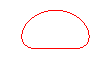
\includegraphics[scale=1,trim={0.2cm 0cm 0cm 0cm},clip]{C1.pdf}& 300 & $250\times750$
				\\
				\hline
				C$_2$ & 40 & 40 & $ 0.4$ & 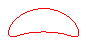
\includegraphics[scale=1,trim={0cm 0cm 0cm 0cm},clip]{C2.pdf}& 400 & $250\times750$
				\\
				\hline
				C$_3$ & 100 & 100 & $ 0.63$ & 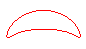
\includegraphics[scale=1,trim={0cm 0cm 0cm 0cm},clip]{C3.pdf}& 500 & $250\times750$
				\\
				\hline
				C$_4$ & 168.5 & 2.2 & $ 0.028$& 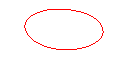
\includegraphics[scale=1,trim={0.3cm 0cm 0cm 0cm},clip]{C4.pdf}& 490 & $160\times1200\times160$
				\\
				\hline
				C$_5$ & 168.5 & 12 & $ 0.028$& 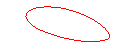
\includegraphics[scale=1,trim={0.3cm 0cm 0cm 0cm},clip]{C5.pdf}& 600 & $160\times1200\times160$
				\\
				\hline
				\hline
			\end{tabular}\label{Table1}
		\end{center}
	\end{table}
	
	The rise of a bubble may exhibit different characteristics and flow dynamics depending on the bubble's non-dimensional parameters, such as the Reynolds and Bond numbers~\cite{Cano-Lozano2016, Hua2007}. In general, three types of rising paths were identified, including rectilinear, spiral, and straight rocking. As shown in Table~\ref{Table1}, five bubble cases are considered in this study. Utilizing the computational setup shown in Figure~\ref{Fig1}(a) with SI-LSM$_{\text{col}}$, three cases of rising bubbles, referred to hereafter as C$_1$, C$_2$, and C$_3$, are simulated on a two-dimensional \textit{axisymmetric} coordinate system. For the computational setup shown in Figure~\ref{Fig1}(b) with CDI, two complex rising cases exhibiting three-dimensional characteristics, referred to as C$_4$ and C$_5$, are simulated on a 3D \textit{Cartesian} coordinate system. Table~\ref{Table1} also summarizes the physical properties of the fluids for the five cases considered here. Cases C$_1$--C$_3$ all exhibit a straight, upward path, but with progressively greater shape variation. C$_1$ remains only weakly deformed, C$_2$ shows a more noticeable deformation, and C$_3$ develops a pronounced skirted shape. While a more complex behavior, including a zigzag rise trajectory from an initial rectilinear path, is obtained in cases C$_4$ and C$_5$, making these two cases challenging for simulation and for the data-driven methods utilized here. For the 2D cases C$_1$--C$_3$, the data-driven analysis is performed from the initial snapshot at $\tau_0$ up to the time at which the bubble first reaches the steady state, together with an additional non-dimensional time interval of 5, leading to 300, 400, and 500 snapshots, respectively. For the 3D cases C$_4$ and C$_5$, all available snapshots from the simulations are used.
	
	\section{Frame of reference}
	\label{framework}
	
	The obtained flow fields from the simulation may be analyzed from different perspectives, including Eulerian, Lagrangian, and moving-reference frameworks. The gas volume-fraction field, denoted here by $\alpha$, representing the bubble's interface, is illustrated in Figure~\ref{Fig2} for case C$_3$ using different frameworks at three time instances. As shown in Figure~\ref{Fig2}(a) for the Eulerian framework, the observer focuses on the fixed grid points with varying flow properties in time. Instead, the Lagrangian framework, shown in Figure~\ref{Fig2}(b), involves tracking the fluid elements, referred to as Lagrangian particles hereafter, from an initial condition; in this case, those in the Eulerian frame at the starting time. The number of Lagrangian particles is identical to the number of Eulerian sampling points, as the tracers are initialized from the Eulerian grid at $\tau_0$. The position of a Lagrangian particle is described through the ordinary differential equation, given as
	
	\begin{figure}[pos=!t]
		\centering
			
\includegraphics[scale=0.5,trim={0cm 0cm 0cm 0cm},clip]{Figure_2.pdf}
		\caption{Instantaneous deformation of the rising bubble at $\tau=0.10,\,4.25,$ and $\,8$ for case C$_3$ in the (a) Eulerian, (b) Lagrangian, and (c) moving-reference frameworks.}
		\label{Fig2}
	\end{figure}
	
	\begin{align}
		\frac{d \mathbf{X}(\tau)}{d \tau} &= \mathbf{U}(\mathbf{X},\tau),
		\label{eq 1}
	\end{align}
	
	\noindent where $\mathbf{X}$ and $\mathbf{U}$ denote the non-dimensional position and velocity vectors of a tracer at time $\tau$, respectively. The velocity vector $\mathbf{U}$ is obtained from the Eulerian DNS velocity field, and Equation~(\ref{eq 1}) is integrated using a first-order (linear) time-integration scheme with a constant snapshot spacing $\Delta\tau$, while at each new particle location the fluid properties, including velocity and gas volume fraction $\alpha$, are linearly interpolated from the Eulerian field, consistent with the numerical treatment adopted by \citet{Yin2023a}. Although in the absence of phase change, a particle within a given phase would ideally remain there, the present tracers are passive, and their motion is governed solely by the continuous velocity field. Because the velocity field does not prevent tracers from crossing the interface, particles initialized near it may move into the opposite phase; therefore, interpolation of the gas volume fraction is required to avoid mislabeling. The particle-tracking algorithm employed here follows the methodology described in~\cite{Majd2024a}. 
	
	In the moving-reference configuration, as shown in Figure~\ref{Fig2}(c), a moving-reference framework is considered. A uniform grid with the same spacing as the Eulerian mesh is initialized at $\tau_0$ within a Region of Interest (ROI) centred on the bubble centroid. The ROI size is chosen as $0.75D\times 1.75D$ for the two-dimensional \textit{axisymmetric} coordinate system, and as a cubic region of size $2D\times 2D \times 2D$ for the three-dimensional \textit{Cartesian} coordinate system. The non-dimensional bubble-centroid position vector is defined by

	\begin{align}
		\mathbf{X}_{\mathrm{cen}}(\tau) &= \frac{1}{V_b(\tau)}\int_{V_b(\tau)}\mathbf{X}\,\mathrm{d}V,
		\label{eq Xcen}
	\end{align}

	\noindent where $V_b(\tau)$ is the instantaneous bubble volume. At each subsequent time step, the grid is translated by the bubble-centroid motion. In the two-dimensional \textit{axisymmetric} case, this translation is applied in the rise direction, whereas in the three-dimensional \textit{Cartesian} case it is applied using the full centroid-velocity vector. In compact form, the position of a moving-reference grid node is written as
	
	\begin{align}
		\mathbf{X}_{\mathrm{M}}(\tau) &= \mathbf{X}_{\mathrm{M}}(\tau_0) + \int_{\tau_0}^{\tau_1} \mathbf{U}_{\mathrm{cen}}(\tau)\,\mathrm{d}\tau,
		\label{eq ME}
	\end{align}
	
	\noindent where $\mathbf{U}_{\mathrm{cen}}(\tau)$ is the non-dimensional bubble centroid-velocity vector obtained from the DNS. Because the centroid-velocity vector is known at each snapshot, the moving-reference grid positions are determined without solving any differential equation; the integral in Equation~(\ref{eq ME}) is evaluated by accumulation as $\mathbf{X}_{\mathrm{M}}(\tau_{k+1}) = \mathbf{X}_{\mathrm{M}}(\tau_k) + \mathbf{U}_{\mathrm{cen}}(\tau_k)\,\Delta\tau$, with the understanding that for the two-dimensional \textit{axisymmetric} case only the rise-direction component is used. Figure~\ref{Fig2}(c) shows the resulting moving origin as a filled red circle bounded within a yellow-bordered ROI. Because the translated grid nodes generally do not coincide with the fixed Eulerian mesh, the fluid properties, including the gas volume fraction $\alpha$ and velocity components, are linearly interpolated in space from the Eulerian DNS field onto the moving-reference grid at each time step. There are some notable advantages of using the moving-reference framework. The grid trajectories are known analytically and therefore require no particle-tracking integration, unlike the Lagrangian approach. It benefits from the localized properties of the flow due to its translational nature and is computationally more efficient, particularly for 3D problems.
	
	In the Eulerian framework, a fixed probe records a rapidly varying time series as the bubble passes through. In contrast, in the Lagrangian and moving-reference frameworks, the observer co-moves with the bubble motion, yielding a smoother, more correlated signal. Both frameworks, therefore, produce datasets that are temporally low-dimensional compared to the Eulerian one, reducing temporal complexity at the expense of determining the coordinates of moving data points by particle tracking in the Lagrangian case and analytically in the moving-reference case.
	
	\section{Data-driven modal decomposition methods}
	\label{Data-driven methods}
	
	Assuming a real-valued dataset $q_i[k]$ sampled at $n_s$ spatial degrees of freedom and using $m$ collected snapshots, the input data matrix $\mathbf{Q}\in \mathbb{R}^{n_s\times m}$ for data-driven analysis is given by
	
	\begin{align}
		\mathbf{Q} = \begin{bmatrix}
			q_{1}[1] & q_{1}[2] & \cdots & q_{1}[m] \\
			q_{2}[1] & q_{2}[2] & \cdots & q_{2}[m] \\
			\vdots & \vdots & \vdots & \vdots \\
			q_{n_s}[1] & q_{n_s}[2] & \cdots & q_{n_s}[m]
		\end{bmatrix}.\label{eq 2}
	\end{align}
	\noindent Equivalently, each snapshot is a column vector $\mathbf{q}_k=[q_1[k],\ldots,q_{n_s}[k]]^T\in\mathbb{R}^{n_s}$, and $\mathbf{Q}=[\mathbf{q}_1,\ldots,\mathbf{q}_m]$.
	\noindent With the input data matrix~(\ref{eq 2}) established, the high-dimensional flow field data sets are decomposed using data-driven methods into low-dimensional spatiotemporal structures, called modes, that represent the dominant flow patterns. In general, decomposition techniques are categorized into energy and frequency-based methods. POD, as an energy-based method, and DMD, as a frequency-based method, are considered in this study. While these methods are closely linked and may exhibit similar flow characteristics when applied to a given dataset, a few differences make them suited to different purposes. For instance, both of these methods are known as ROMs and can therefore be used to reconstruct the original data using only a few modes. POD and DMD are also known as equation-free methods, meaning they do not rely on the governing equations of the system. This allows them to be applied to numerical and experimental datasets.
	
	Regarding the discrepancies, only DMD can predict the system's future state when benefiting from ROMs. Each DMD mode is associated with a single frequency, whereas in POD, multiple frequencies may correspond to multiple scales for a given mode. With respect to reconstruction, POD is more straightforward because the extracted modes are arranged in descending order of energy. This facilitates the selection of the most relevant modes. In contrast, DMD reconstruction relies on the contribution of each mode's amplitude. A few criteria for obtaining the DMD amplitudes will be discussed further in Section~\ref{DMD amplitudes}.  
	
	\subsection{POD}
	\label{POD}
	
	This energy-based method can optimally extract the most energetic feature of the flow through dimensional reduction. In practice, one way of dimensional reduction is by taking the singular value decomposition (SVD) of $\mathbf{Q}$, given as
	\begin{align}
		\mathbf{Q} = \mathbf{\Phi} \mathbf{\Sigma} \mathbf{\Psi}^T ,\label{eq 3}
	\end{align}
	\noindent where $\mathbf{\Phi} \in \mathbb{R}^{n_s\times m}$ holds the spatial modes and $\mathbf{\Psi}\in \mathbb{R}^{m\times m}$ contains the temporal ones. Note that in the SVD computation, $\mathbf{\Sigma}\in \mathbb{R}^{m\times m}$ is a diagonal matrix holding singular values of $\mathbf{Q}$ in descending order, reflecting the importance of each mode. In most cases, $\mathbf{Q}$ is a tall and skinny matrix with millions of rows and thousands of columns, making the SVD computation costly and impractical. An alternative approach is the method of snapshots proposed by \citet{Sirovich1987} by considering the right eigenvalue problem of the matrix $\mathbf{Q}^T\mathbf{Q}$ with a much smaller size of $m\times m$, given as 
	
	\begin{align}
		\mathbf{Q}^T\mathbf{Q}\boldsymbol{\psi} _j = \lambda _j \boldsymbol{\psi} _j.\label{eq 4}
	\end{align}
	
	\noindent By solving Equation~(\ref{eq 4}) for eigenvalues $\lambda _j$ and their corresponding eigenvectors $\boldsymbol{\psi} _j$, the spatial modes $\boldsymbol{\phi} _j$, with $j\in [1,~.~.~.~, m]$ are determined as
	
	\begin{align}
		\boldsymbol{\phi} _j = \mathbf{Q} \boldsymbol{\psi} _j \frac{1}{\sqrt{\lambda _j}}.\label{eq 5}
	\end{align}
	
	\noindent It should be noted that the singular values of the SVD decomposition in Equation~(\ref{eq 3}) are related to the eigenvalues obtained in Equation~(\ref{eq 4}) by $\sigma_j = \sqrt{\lambda_j}$. The snapshot method has been widely used due to the smaller size of the correlation matrix. However, one may still use the SVD-based method, as it is reliable and accurate even in the presence of roundoff errors. POD modes are then ranked by their energy levels, as given by the eigenvalues. Thus, incoherent noise with low energy levels appears in the higher-order modes.
	
	\subsection{DMD}
	\label{DMD}
	
	This decomposition technique can identify spatial features and their dynamics. Each mode is associated with a single oscillation frequency and decay/growth rates given by the corresponding eigenvalues. Many mathematical formulations exist in the literature, amongst which the algorithm-1 in the work of \citet{H.Tu2014} is presented here. It involves four main steps, including
	\begin{itemize}
		\item[1.] The arrangement of input data matrices $\mathbf{Q}'$ and $\mathbf{Q}''\in \mathbb{R}^{n_{s}\times (m-1)}$:
		\begin{subequations}\label{eq 6}
			\begin{align}
				\mathbf{Q}' = [\mathbf{q}_1,\mathbf{q}_2,\ldots,\mathbf{q}_{m-1}], \label{eq 6a} \\
				\mathbf{Q}'' = [\mathbf{q}_2,\mathbf{q}_3,\ldots,\mathbf{q}_{m}].\label{eq 6b}
			\end{align}
		\end{subequations}
		where $\mathbf{q}_k=[q_1[k],\ldots,q_{n_s}[k]]^T\in\mathbb{R}^{n_s}$ denotes the snapshot vector at time index $k$.
		\item[2.] Computing the truncated SVD by considering only a reduced $r$ number of modes (truncation rank, $r\le m-1$):
		\begin{align}
			\mathbf{Q}' \approx \mathbf{\Phi}_r\mathbf{\Sigma} _r \mathbf{\Psi}_r^T, \label{eq 7}
		\end{align}
		where $\mathbf{\Phi}_r$, $\mathbf{\Sigma}_r$, and $\mathbf{\Psi}_r$ are the truncated SVD factors of $\mathbf{Q}'$.
		\item[3.] Solving the eigenvalue problem of:
		\begin{align}
			\tilde{A} \mathbf{w}_j = \mu_j \mathbf{w}_j, \label{eq 8}
		\end{align}
		where $\tilde{A}=\mathbf{\Phi}_r^T \mathbf{Q}'' \mathbf{\Psi}_r \mathbf{\Sigma}_r^{-1}$. The eigenvalues $\mu_j$ of $\tilde{A}$ are in general complex; $|\mu_j|$ determines the discrete-time growth/decay per snapshot and $\arg(\mu_j)$ sets the oscillation frequency.
		
		\item[4.] Determining the spatial modes as follows:
		\begin{align}
			\boldsymbol{\varphi} _j = \mathbf{\Phi}_r\mathbf{w}_j. \label{eq 9}
		\end{align}
		
	\end{itemize}
	It is important to note that, unlike POD, where the importance of the modes is characterized by their energy content (eigenvalues), the DMD modes are typically ranked by their amplitudes. 
	
	\subsubsection{DMD amplitudes}
	\label{DMD amplitudes}
	
	The reconstruction procedure in DMD requires determining the amplitudes corresponding to each DMD mode. The most straightforward but less accurate approach is to compute the initial amplitudes as follows \cite{Kutz2016}
	
	\begin{align}
		\mathbf{q}(\tau)\approx \sum_{j=1}^{r} \boldsymbol{\varphi}_j e^{\omega_j \tau} b_j = \mathbf{\Phi}_{DMD}\,\exp (\mathbf{\Omega}\, \tau)\,\mathbf{b}.
		\label{eq 10}
	\end{align}
	
	\noindent where $\mathbf{q}(\tau)\in\mathbb{R}^{n_s}$ is the reconstructed snapshot at time $\tau=k\Delta\tau$, with $k=0,1,\ldots,m-1$ and a constant snapshot spacing $\Delta\tau$. Here, $\mathbf{\Phi}_{DMD}=[\boldsymbol{\varphi}_1,\ldots,\boldsymbol{\varphi}_r]$ is the matrix of DMD modes, $\mathbf{\Omega}=\mathrm{diag}(\omega_1,\ldots,\omega_r)$, and the continuous-time eigenvalues are given by $\omega_j=\ln(\mu_j)/\Delta\tau$. The vector $\mathbf{b}\in\mathbb{C}^{r}$ contains the initial modal amplitudes, commonly estimated as $\mathbf{b}=\mathbf{\Phi}_{DMD}^{\dagger}\mathbf{q}(0)$, where the superscript $\dagger$ denotes the Moore--Penrose pseudoinverse. These amplitudes reflect the importance and relevance of each mode to the system's overall dynamics. Therefore, one may assume that only DMD modes with the highest amplitudes should be included in the reconstruction. Since the amplitudes are obtained by projecting the first snapshot onto the DMD modes, the reconstruction is more likely to be accurate for early-stage flow features. This might also lead to incomplete reconstruction in cases where structures become more important as the system evolves. 
	
	An alternative approach to obtain the DMD amplitudes involves solving an optimization problem, where a trade-off is made between the sparsity of the included modes and the accuracy of the reconstruction. This strategy, proposed by \citet{Jovanovic2014}, can efficiently retain the most relevant modes with their actual amplitudes by solving the optimization problem $\min\,\|\mathbf{Q}' - \mathbf{\Phi}_{DMD}\, \mathbf{B}\, \mathbf{Z}_{\mu}\|_F^2$, where $\|\cdot\|_F$ denotes the Frobenius norm. Here, $\mathbf{B}=\mathrm{diag}(\mathbf{b})$ is the diagonal matrix of modal amplitudes and $\mathbf{Z}_{\mu}$ is the Vandermonde matrix constructed from the DMD eigenvalues $\mu_j$. Using SVD properties, the definition of the DMD modes, and some algebra, the result can be written in a quadratic form that is solved using the alternating direction method of multipliers technique. Readers are referred to previously published literature \cite{Jovanovic2014,Schmid2023} for more details on this method. 
	
	\subsection{Input data matrix structure}
	
	As described in Section~\ref{framework}, the flow fields obtained from the DNS can be represented in three reference frames, namely Eulerian (E), Lagrangian (L), and moving frame (M). Different observation variables extracted from these frames may be used as inputs to data-driven algorithms, depending on the physical property of interest. In this study, two primary observation variables, the gas volume fraction ($\alpha$) and the velocity field, are considered. The gas volume fraction is used to characterize bubble deformation, track the interface, and determine the rising trajectory. The velocity field, on the other hand, provides information about the flow dynamics and the spatiotemporal structures developing in the bubble wake. Both quantities are required for estimating global properties such as the rise velocity. 	Accordingly, the combination of reference frame and the decomposition method defines a family of distinct input datasets for the subsequent data-driven analysis, referred to here using a compact notation based on the selected frame and method. For example, the decomposition of the Eulerian field using POD is denoted as E-POD.
	
	For a selected framework, let $n_s$ denote the number of sampling points and $m$ the number of collected snapshots. Each snapshot of the observation field is first reshaped into a column vector. Stacking $m$ snapshots then forms the input data matrices.
	\[
	\mathbf{A}=
	\begin{bmatrix}
		\mathbf{\alpha}_1 & \mathbf{\alpha}_2 & \cdots & \mathbf{\alpha}_m
	\end{bmatrix}
	\in \mathbb{R}^{n_s \times m},
	\qquad
	\mathbf{V}=
	\begin{bmatrix}
		\mathbf{U}_1 & \mathbf{U}_2 & \cdots & \mathbf{U}_m
	\end{bmatrix}
	\in \mathbb{R}^{dn_s \times m},
	\]
	where $\mathbf{A}$ and $\mathbf{V}$ denote the gas volume fraction and velocity data matrices, respectively, with $\mathbf{\alpha}_k$ denoting the gas volume fraction snapshot vector and $\mathbf{U}_k$ denoting the non-dimensional velocity snapshot vector at time index $k$, and $d=2$ for the two-dimensional axisymmetric cases and $d=3$ for the three-dimensional Cartesian cases. In the notation introduced in Section~\ref{Data-driven methods}, the generic input matrix $\mathbf{Q}$ therefore represents either $\mathbf{A}$ or $\mathbf{V}$, depending on the selected observable. The matrices are decomposed independently using the selected data-driven method, and the truncated reconstructions with $r$ modes are denoted by $\mathbf{A}^{(r)}$ and $\mathbf{V}^{(r)}$. In the Lagrangian framework, the coordinate matrix of tracer locations must also be retained to represent the reconstructed fields at their corresponding positions. The coordinate matrix is written as
	\[
	\mathbf{P}=
	\begin{bmatrix}
		\mathbf{X}_1 & \mathbf{X}_2 & \cdots & \mathbf{X}_m
	\end{bmatrix}
	\in \mathbb{R}^{dn_s \times m},
	\]
	where $\mathbf{X}_k$ contains the non-dimensional tracer-position snapshot vector at time index $k$. In contrast, the coordinates of the Eulerian grid remain fixed and therefore require no reconstruction, while the coordinates in the moving-reference framework are known analytically from the centroid motion described in Section~\ref{framework}. 
	
	%%%%%%%%%%%%%%%%%%%%%%%%%%%%%________Figure_3___________%%%%%%%%%%%%%%%%%%%%%
	\begin{figure}[pos=!tbp]
		\centering
			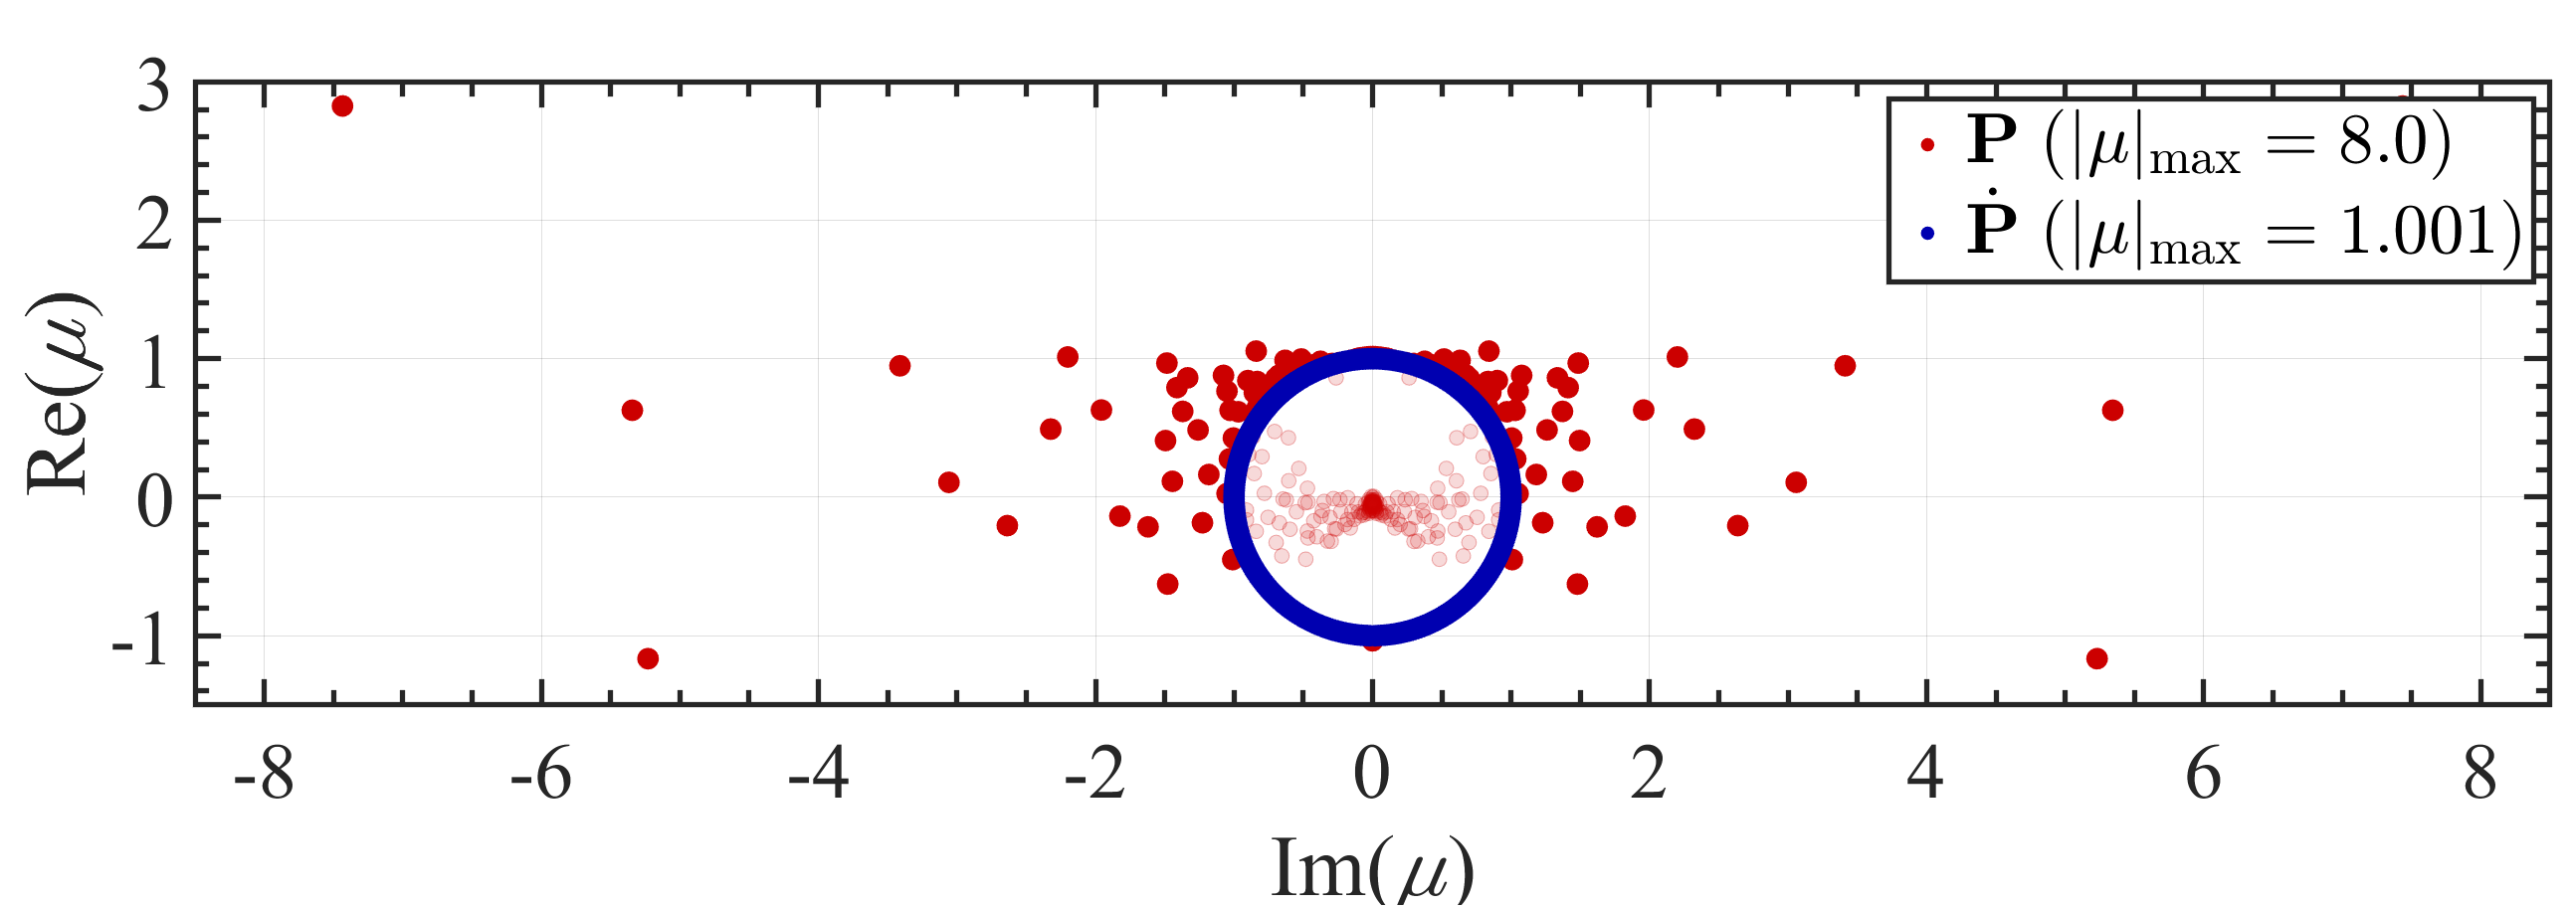
\includegraphics[scale=0.25,trim={0cm 0cm 0cm 0cm},clip]{Figure_3.pdf}
		\caption{Distribution of the DMD eigenvalues $\mu$ in the complex plane for the Lagrangian position matrix $\mathbf{P}$ and its time derivative $\dot{\mathbf{P}}$. Red and blue markers denote the eigenvalues obtained from $\mathbf{P}$ and $\dot{\mathbf{P}}$, respectively.}
		\label{Fig3}
	\end{figure}
	%%%%%%%%%%%%%%%%%%%%%%%%%%%%%________Figure_3_end___________%%%%%%%%%%%%%%%%%%%%%
	
	A specific preprocessing step is required for the Lagrangian coordinate matrix. Applying DMD directly to the position matrix $\mathbf{P}$ yields a significant number of modes with $|\mu|>1$, as shown in Figure~\ref{Fig3}. In other words, $\dot{\mathbf{P}}$ describes the instantaneous particle motion, whereas $\mathbf{P}$ describes the particle positions after that motion has accumulated over time. Consequently, persistent translational drift and other low-frequency kinematic trends accumulate in $\mathbf{P}$ across snapshots, and DMD represents this drift through discrete-time modes with amplified magnitude. In the DMD reconstruction, such modes enter the Vandermonde matrix $\mathbf{Z}_{\mu}$ through powers of $\mu_j$, so eigenvalues with $|\mu_j|>1$ produce rapid temporal growth and may lead to numerical overflow. For this reason, the Lagrangian coordinate observable is analysed through the time-derivative of the position matrix, $\dot{\mathbf{P}}$, instead of through $\mathbf{P}$ itself. This preprocessing is used for both POD and DMD in the present study, while the stability motivation arises directly from the DMD eigenspectrum. As shown in Figure~\ref{Fig3}, differentiation suppresses the accumulated drift. It shifts the observable toward the instantaneous Lagrangian kinematics, yielding an eigenspectrum concentrated in the stable neighbourhood of the unit circle and therefore a more numerically robust representation. The reconstructed position matrix is then obtained by integrating the reconstructed time-derivative $\dot{\mathbf{P}}$ in time. For the other observables considered in this study, namely the gas volume fraction and velocity fields, temporal mean subtraction is used.
	
	\section{Results and discussion}
	\label{Results and discussion}
	
	
	\subsection{Reconstruction error of observation variables}
	
	In this section, different flow variables, including the velocity field, gas volume fraction, and the time derivative of the Lagrangian position matrix, are reconstructed using the POD and DMD methods in Eulerian, Lagrangian, and moving-reference frameworks. For field-reconstruction-accuracy analysis, only cases C$_1$ (Re$=20$, Bo$=20$) and C$_3$ (Re$=100$, Bo$=100$) are shown, representing the least and most deforming two-dimensional bubbles considered in this study. The accuracy of the reconstructed field is evaluated by means of the Frobenius norm of the difference between the original input data matrix and its approximation. Using the properties of SVD, the relative reconstruction errors of a field using POD and DMD for $r$ number of modes are simplified and given by:
	
	%%%%%%%%%%%%%%%%%%%%%%%%%%%%%________Figure_3___________%%%%%%%%%%%%%%%%%%%%%
	\begin{figure}[pos=!t]
		\centering
			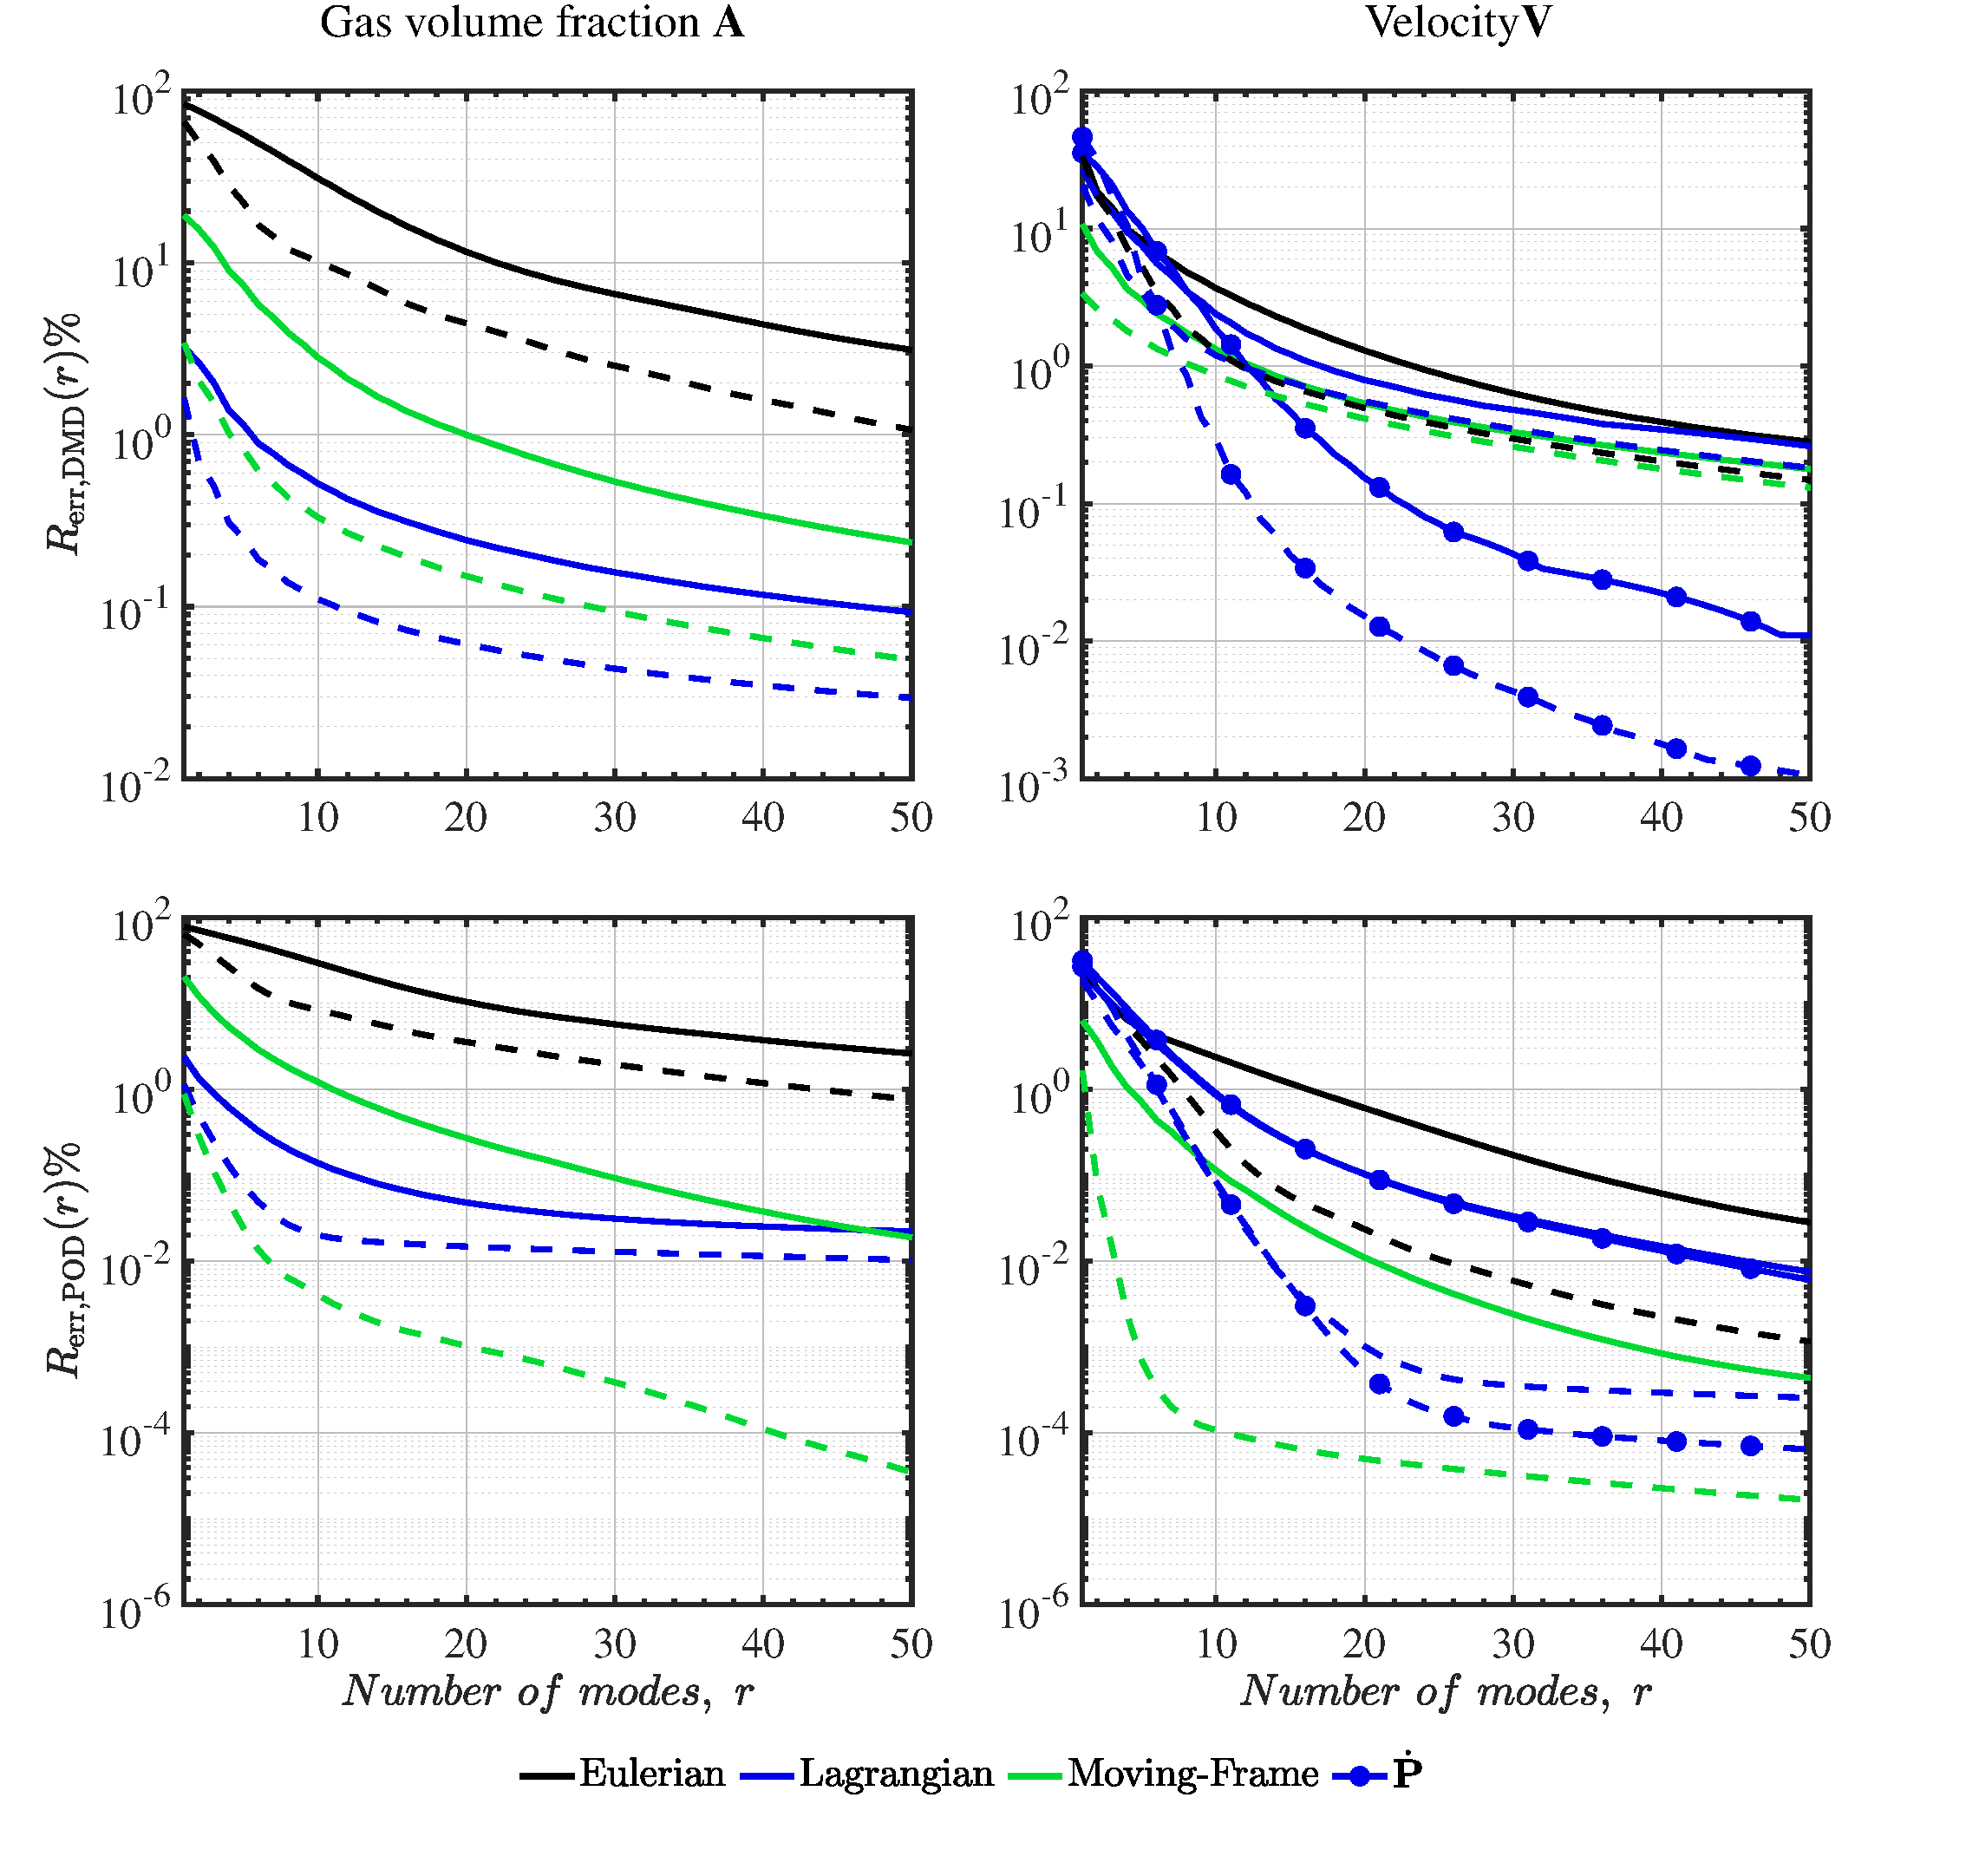
\includegraphics[scale=0.38,trim={0cm 0cm 0cm 0cm},clip]{Figure_4.pdf}
		\caption{Relative reconstruction error for the gas volume fraction and velocity fields in Eulerian, Lagrangian, and moving-reference frameworks for rising bubble cases C$_1$ (dashed lines) and C$_3$ (solid lines). The top and bottom rows correspond to DMD and POD, respectively; the left and right columns correspond to the gas volume fraction and velocity fields.}
		\label{Fig4}
	\end{figure}
	%%%%%%%%%%%%%%%%%%%%%%%%%%%%%________Figure_3_end___________%%%%%%%%%%%%%%%%%%%%%
	
	\begin{subequations}\label{eq 12}
		\begin{align}
			R_{\mathrm{err},\mathrm{POD}}(r) = \frac{\lVert\mathbf{Q} - \mathbf{Q}^{(r)}\rVert_F^2}{\lVert\mathbf{Q}\rVert_F^2} = \frac{\sum\limits_{j=r+1}^m \sigma_j^2}{\sum\limits_{j=1}^m \sigma_j^2}, \label{eq 16a} \\
			R_{\mathrm{err},\mathrm{DMD}}(r) = \frac{\lVert\mathbf{Q}' - \mathbf{\Phi}_{\mathrm{DMD}}\mathbf{B}_r\mathbf{Z}_{\mu}\rVert_F^2}{\lVert\mathbf{Q}'\rVert_F^2}.\label{eq 16b}
		\end{align}\label{eq 16}
	\end{subequations}
	
	\noindent In Equation~(\ref{eq 16}), $\mathbf{Q}$ denotes the selected input matrix, namely $\mathbf{A}$ for the gas volume fraction field, $\mathbf{V}$ for the velocity field, or $\dot{\mathbf{P}}$ for the time-derivative of the Lagrangian position matrix, and $\mathbf{Q}^{(r)}$ is its rank-$r$ reconstruction. The above errors in the reduced space are computationally less expensive than working with the full input data matrix of size $n_s \times m$. Preceding the discussion on the efficiency of reconstruction, it is necessary to emphasize that two types of errors are assessed in this study. One is already introduced in Equation~(\ref{eq 16}), while the other is the conventional root-mean-square deviation (RMSD) used for scalar variables. The former is used for the overall evaluation of the reconstructed field, while the latter is applied to quantitative time-varying parameters such as the rise velocity and circularity of the bubble, which will be discussed further in section~\ref{Bubble interface}. This distinction is essential in the present study as a framework may yield a very compact reconstruction of its sampled field while still failing to preserve the physically meaningful bubble shape or rise properties derived from that field.
	
	The error of the reconstructed fields is evaluated using Equation~(\ref{eq 16}) in the Eulerian, Lagrangian, and moving-reference frameworks, employing POD and DMD techniques, as shown in Figure~\ref{Fig4} for cases C$_1$ and C$_3$. A preliminary assessment of the results suggests that the choice of reference frame has a far stronger influence on the reconstruction error than the choice of method. For instance, the results of bubble C$_1$ with small deformation for the gas volume fraction matrix $\mathbf{A}$ show that the Eulerian POD and DMD reconstructions yield errors of approximately $8.4\%$ and $10.1\%$ with 10 modes. In contrast, at the same rank, the most accurate results are achieved in the moving-reference and Lagrangian frameworks with POD, where the reconstruction errors are as small as $0.004\%$ and $0.020\%$, respectively. In the case of DMD applied to $\mathbf{A}$ in the moving-reference and Lagrangian frameworks, the relative reconstruction errors are approximately $0.33\%$ and $0.11\%$ at 10 modes, notably higher than their POD counterparts. The effectiveness of the Lagrangian and moving-reference frameworks stems from the way flow dynamics are represented in snapshot data. In the Eulerian frame, the translating bubble interface appears as a sweeping spatial pattern requiring many modes to represent. In contrast, the Lagrangian and moving-reference frameworks co-move with the bubble, rendering the interface nearly stationary and inherently low-rank. The POD-over-DMD gap is a consequence of DMD's intrinsic assumption of linear dynamics, which constrains each mode to a fixed frequency and exponential growth rate. POD imposes no such temporal structure and, by construction, provides the globally optimal low-rank approximation in the least-squares sense for any given number of modes.
	
	The analysis of the relative reconstruction error for bubble C$_3$ supports the established patterns for C$_1$. However, due to the greater deformation in this case, a higher relative reconstruction error is observed with the same number of modes compared to case C$_1$. The Eulerian framework becomes markedly less efficient, with errors of $29.5\%$ for the POD and $31.1\%$ for the DMD at 10 modes for the reconstruction of $\mathbf{A}$. Whereas the Lagrangian framework remains the most compact with $0.14\%$ for POD and $0.52\%$ for DMD at 10 modes. This can be observed in the moving-reference framework as well, with reconstruction errors of $1.2\%$ and $2.8\%$ for POD and DMD, respectively, at 10 modes, which are larger than those for C$_1$ since the rigid-frame translation can no longer fully compensate for the shape changes of the strongly deforming bubble.
	
	The velocity field is notably more compact than the gas volume fraction field, requiring far fewer modes for accurate reconstruction in the Eulerian frame. For example, the Eulerian POD reconstruction of $\mathbf{V}$ yields errors of $0.32\%$ and $2.4\%$ for C$_1$ and C$_3$ at 10 modes, compared with $8.4\%$ and $29.5\%$ for the corresponding Eulerian POD reconstruction of $\mathbf{A}$. The moving-reference framework provides the clearest improvement for the velocity field. By removing the mean advection, only the residual wake fluctuations remain, which are inherently low-rank. For example, the moving-reference POD reconstruction of $\mathbf{V}$ reduces the reconstruction error to $0.11\%$ for C$_3$ at 10 modes.
	
	Regarding the time-derivative of the Lagrangian position matrix $\dot{\mathbf{P}}$, which is defined exclusively in the Lagrangian framework, the reconstruction error is notably compact for both POD and DMD. The POD reconstruction of $\dot{\mathbf{P}}$ yields errors of $0.083\%$ and $0.896\%$ for C$_1$ and C$_3$ at 10 modes, while the corresponding DMD reconstruction yields $0.293\%$ and $1.850\%$, respectively. The time derivative of the Lagrangian position matrix shares the same kinematic nature as the velocity field and therefore exhibits a similarly low-rank spectral structure. 
	
	Overall, based on the analysis of the relative reconstruction error, one may conclude that the reference frame is the primary driver of reconstruction efficiency, with the Lagrangian and moving-reference frameworks consistently outperforming the Eulerian one, an advantage that becomes more pronounced as bubble deformation increases. The choice of method between POD and DMD is a secondary but consistent effect that uniformly favours POD, particularly at low rank. At the same time, the present field-based comparison should be interpreted only as a measure of compactness of the sampled representation; the following subsections show that physical reliability must be judged from the reconstructed rise properties themselves.
	
	\subsection{Bubble interface}
	\label{Bubble interface}
	
	\begin{figure}[pos=!t]
		\centering
		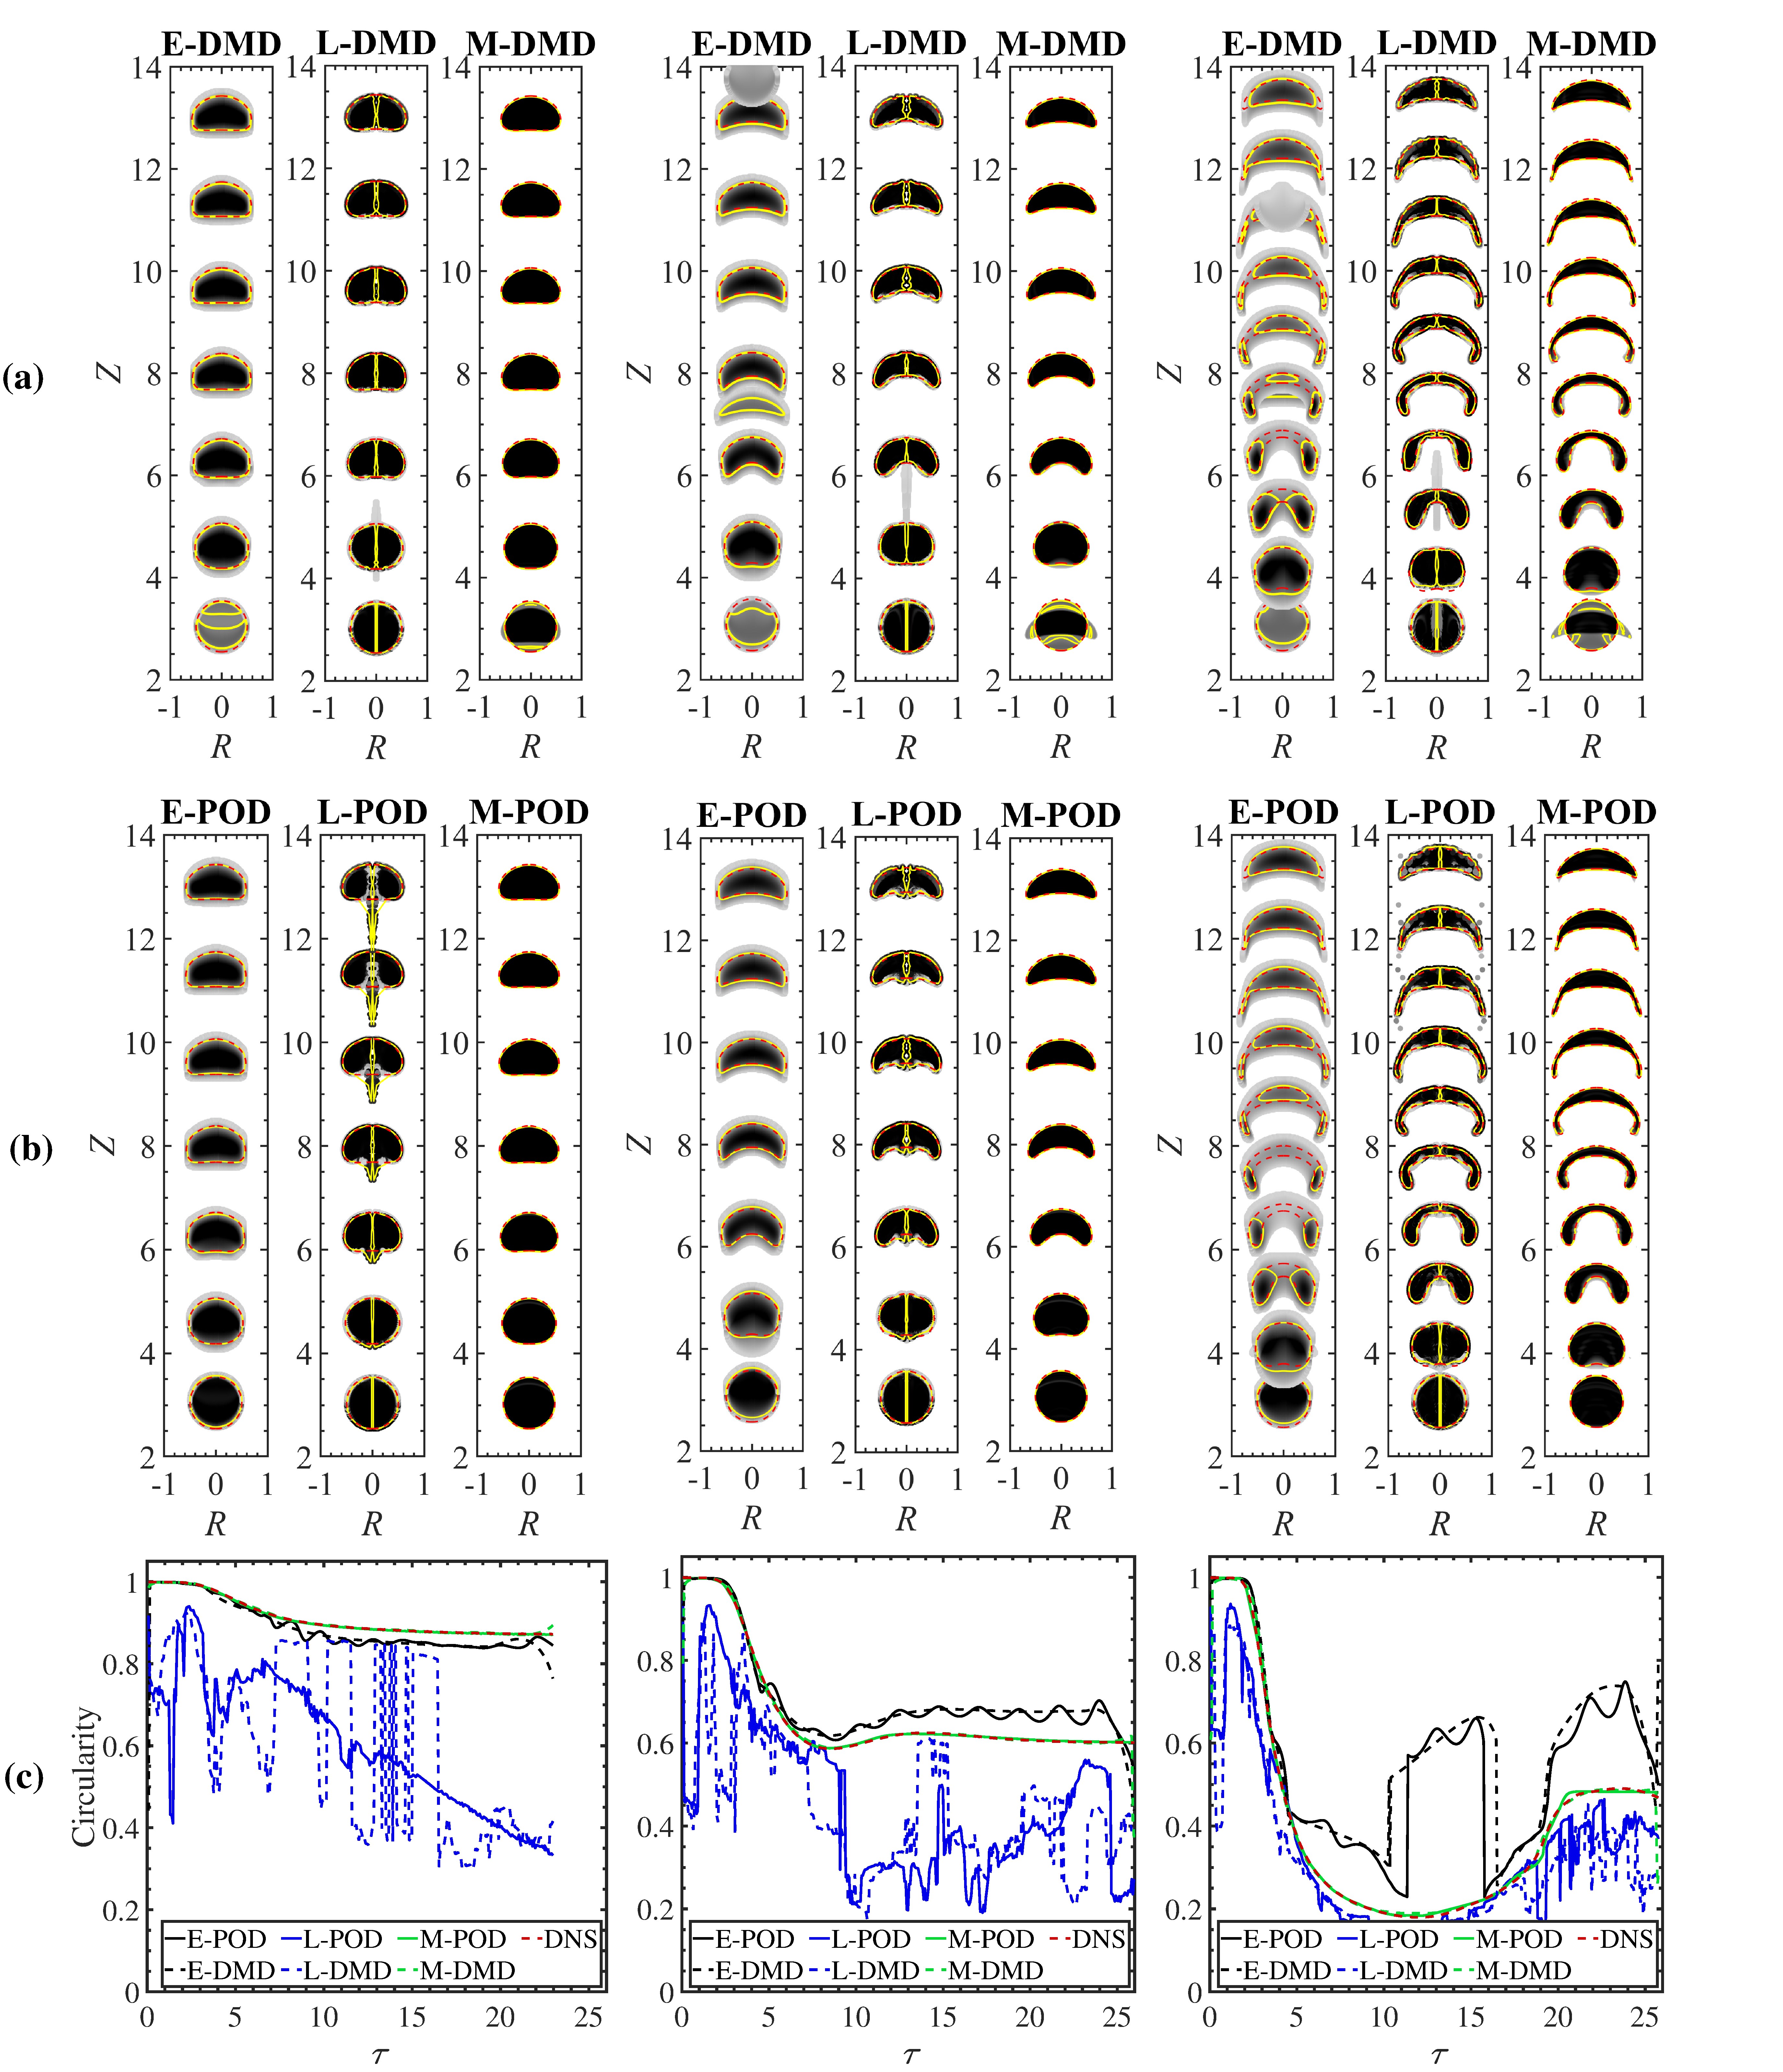
\includegraphics[scale=0.183,trim={0cm 0cm 6cm 0cm},clip]{Figure_5.pdf}
		\caption{Temporal evolution of the bubble interface reconstructed with 10 modes for cases C$_1$--C$_3$. Panels (a), (b), and (c) correspond to DMD, POD, and the associated circularity profiles, respectively, with cases C$_1$, C$_2$, and C$_3$ shown from left to right. The interface snapshots are mirrored about $Z=0$ and successively shifted by $0.025D$ in the axial direction. Yellow solid and red dashed lines indicate reconstructed and DNS $\alpha=0.5$ iso-contours, respectively.}
		\label{Fig5}
		\vspace{-2pt}
	\end{figure}
	
	An overall analysis of the relative reconstruction error shows that, in terms of field reconstruction efficiency, the moving-reference and Lagrangian frameworks outperform the Eulerian framework. However, their accuracy in approximating the bubble interface and rise properties has not yet been examined directly. To address this, the bubble interface, its rise velocity, and circularity are approximated for C$_1$, C$_2$, and C$_3$ using 10 modes during the rising process. The truncation rank of 10 is selected as a consistent, low-order choice to enable fair comparisons across frameworks and to retain a compact representation even in more complex cases. Since this subsection focuses on the gas volume fraction field, the discussion refers directly to reconstructions of the matrix $\mathbf{A}$ in the Eulerian, Lagrangian, and moving-reference frameworks.
	
	Circularity, as a quantitative geometric metric, provides a precise criterion to assess the accuracy of the reconstructed bubble shape~\cite{Hysing2009}. A value of 1 corresponds to a perfectly circular bubble, while lower values indicate deformation. However, in the present results, circularity alone is still insufficient to assess reconstruction quality, because some methods may yield a comparatively small field reconstruction error while still exhibiting visible interface distortions or discontinuities. This issue is most evident in the Lagrangian framework, where irregular interfaces and strongly fluctuating circularity profiles are observed. Therefore, the reconstructed interfaces in the first and second rows of Figure~\ref{Fig5} are interpreted together with the circularity histories in the third row, Figure~\ref{Fig5}(c).

	The Eulerian framework is the least reliable for interface reconstruction. In the first-row DMD panels of Figure~\ref{Fig5}(a), the interface is only partially recovered for C$_1$ and C$_2$, and the reconstruction becomes inadequate for the more deforming case C$_3$. The second-row POD panels in Figure~\ref{Fig5}(b) improve the interface approximation, but visible distortion remains. The circularity data in Figure~\ref{Fig5}(c) confirm this trend. More precisely, the RMSD errors for C$_1$, C$_2$, and C$_3$ are 4.57\%, 7.54\%, and 50.11\% for E-DMD, compared with 2.75\%, 6.82\%, and 43.49\% for E-POD. Thus, POD consistently outperforms DMD in the Eulerian framework, but both deteriorate substantially as bubble deformation increases.
	
	The Lagrangian framework yields much smaller field-reconstruction errors than the Eulerian one, but this does not translate into the most accurate interface. In both the first and second rows of Figure~\ref{Fig5}, the Lagrangian reconstructions exhibit irregular shapes and false signs of breakup. The circularity histories in Figure~\ref{Fig5}(c) show that this effect is severe for C$_1$ and C$_2$. The RMSD errors are 39.00\% and 38.98\% for L-DMD, and 36.65\% and 37.41\% for L-POD. For C$_3$, the Lagrangian circularity error decreases to 28.22\% for DMD and 21.82\% for POD. This explains why the very small relative reconstruction errors of the Lagrangian gas volume fraction field, namely 0.11\%, 0.19\%, and 0.52\% for DMD and 0.020\%, 0.057\%, and 0.14\% for POD, are not reliable to assess the actual interface quality. Equation~(\ref{eq 16a}) measures only the projection error of the data-driven reconstruction relative to its Lagrangian input data; it does not include the additional geometric error. Accordingly, the Lagrangian framework should be interpreted here as compact but not physically robust for interface-based analysis, despite its low field-reconstruction error.
	
	The moving-reference framework provides the most accurate and consistent interface reconstruction. In the second-row POD panels of Figure~\ref{Fig5}(b), the bubble interface remains close to DNS throughout the rising process for all three cases, and the circularity curves in Figure~\ref{Fig5}(c) confirm this quantitatively with RMSD errors of only 0.13\%, 0.27\%, and 1.42\% for C$_1$, C$_2$, and C$_3$, respectively. The corresponding field-reconstruction errors are also very small, namely 0.004\%, 0.053\%, and 1.22\% at 10 modes. M-DMD performs less accurately than M-POD, but it remains markedly better than the Eulerian and Lagrangian alternatives in terms of interface fidelity. Its circularity RMSD errors are 0.32\%, 2.71\%, and 6.15\% for C$_1$, C$_2$, and C$_3$, respectively, with relative field reconstruction errors of 0.33\%, 1.00\%, and 2.82\%. The main weakness of M-DMD is the greater deviation from DNS at early times, and this deficiency becomes more pronounced as bubble deformation increases. Overall, the present interface and circularity data indicate that M-POD is the most reliable approach in this section, while M-DMD is the second-best compromise between interface accuracy and compactness.
	
	\subsection{Rise velocity}
	\label{Rise velocity}
	
	\begin{figure}[pos=!t]
		\centering
		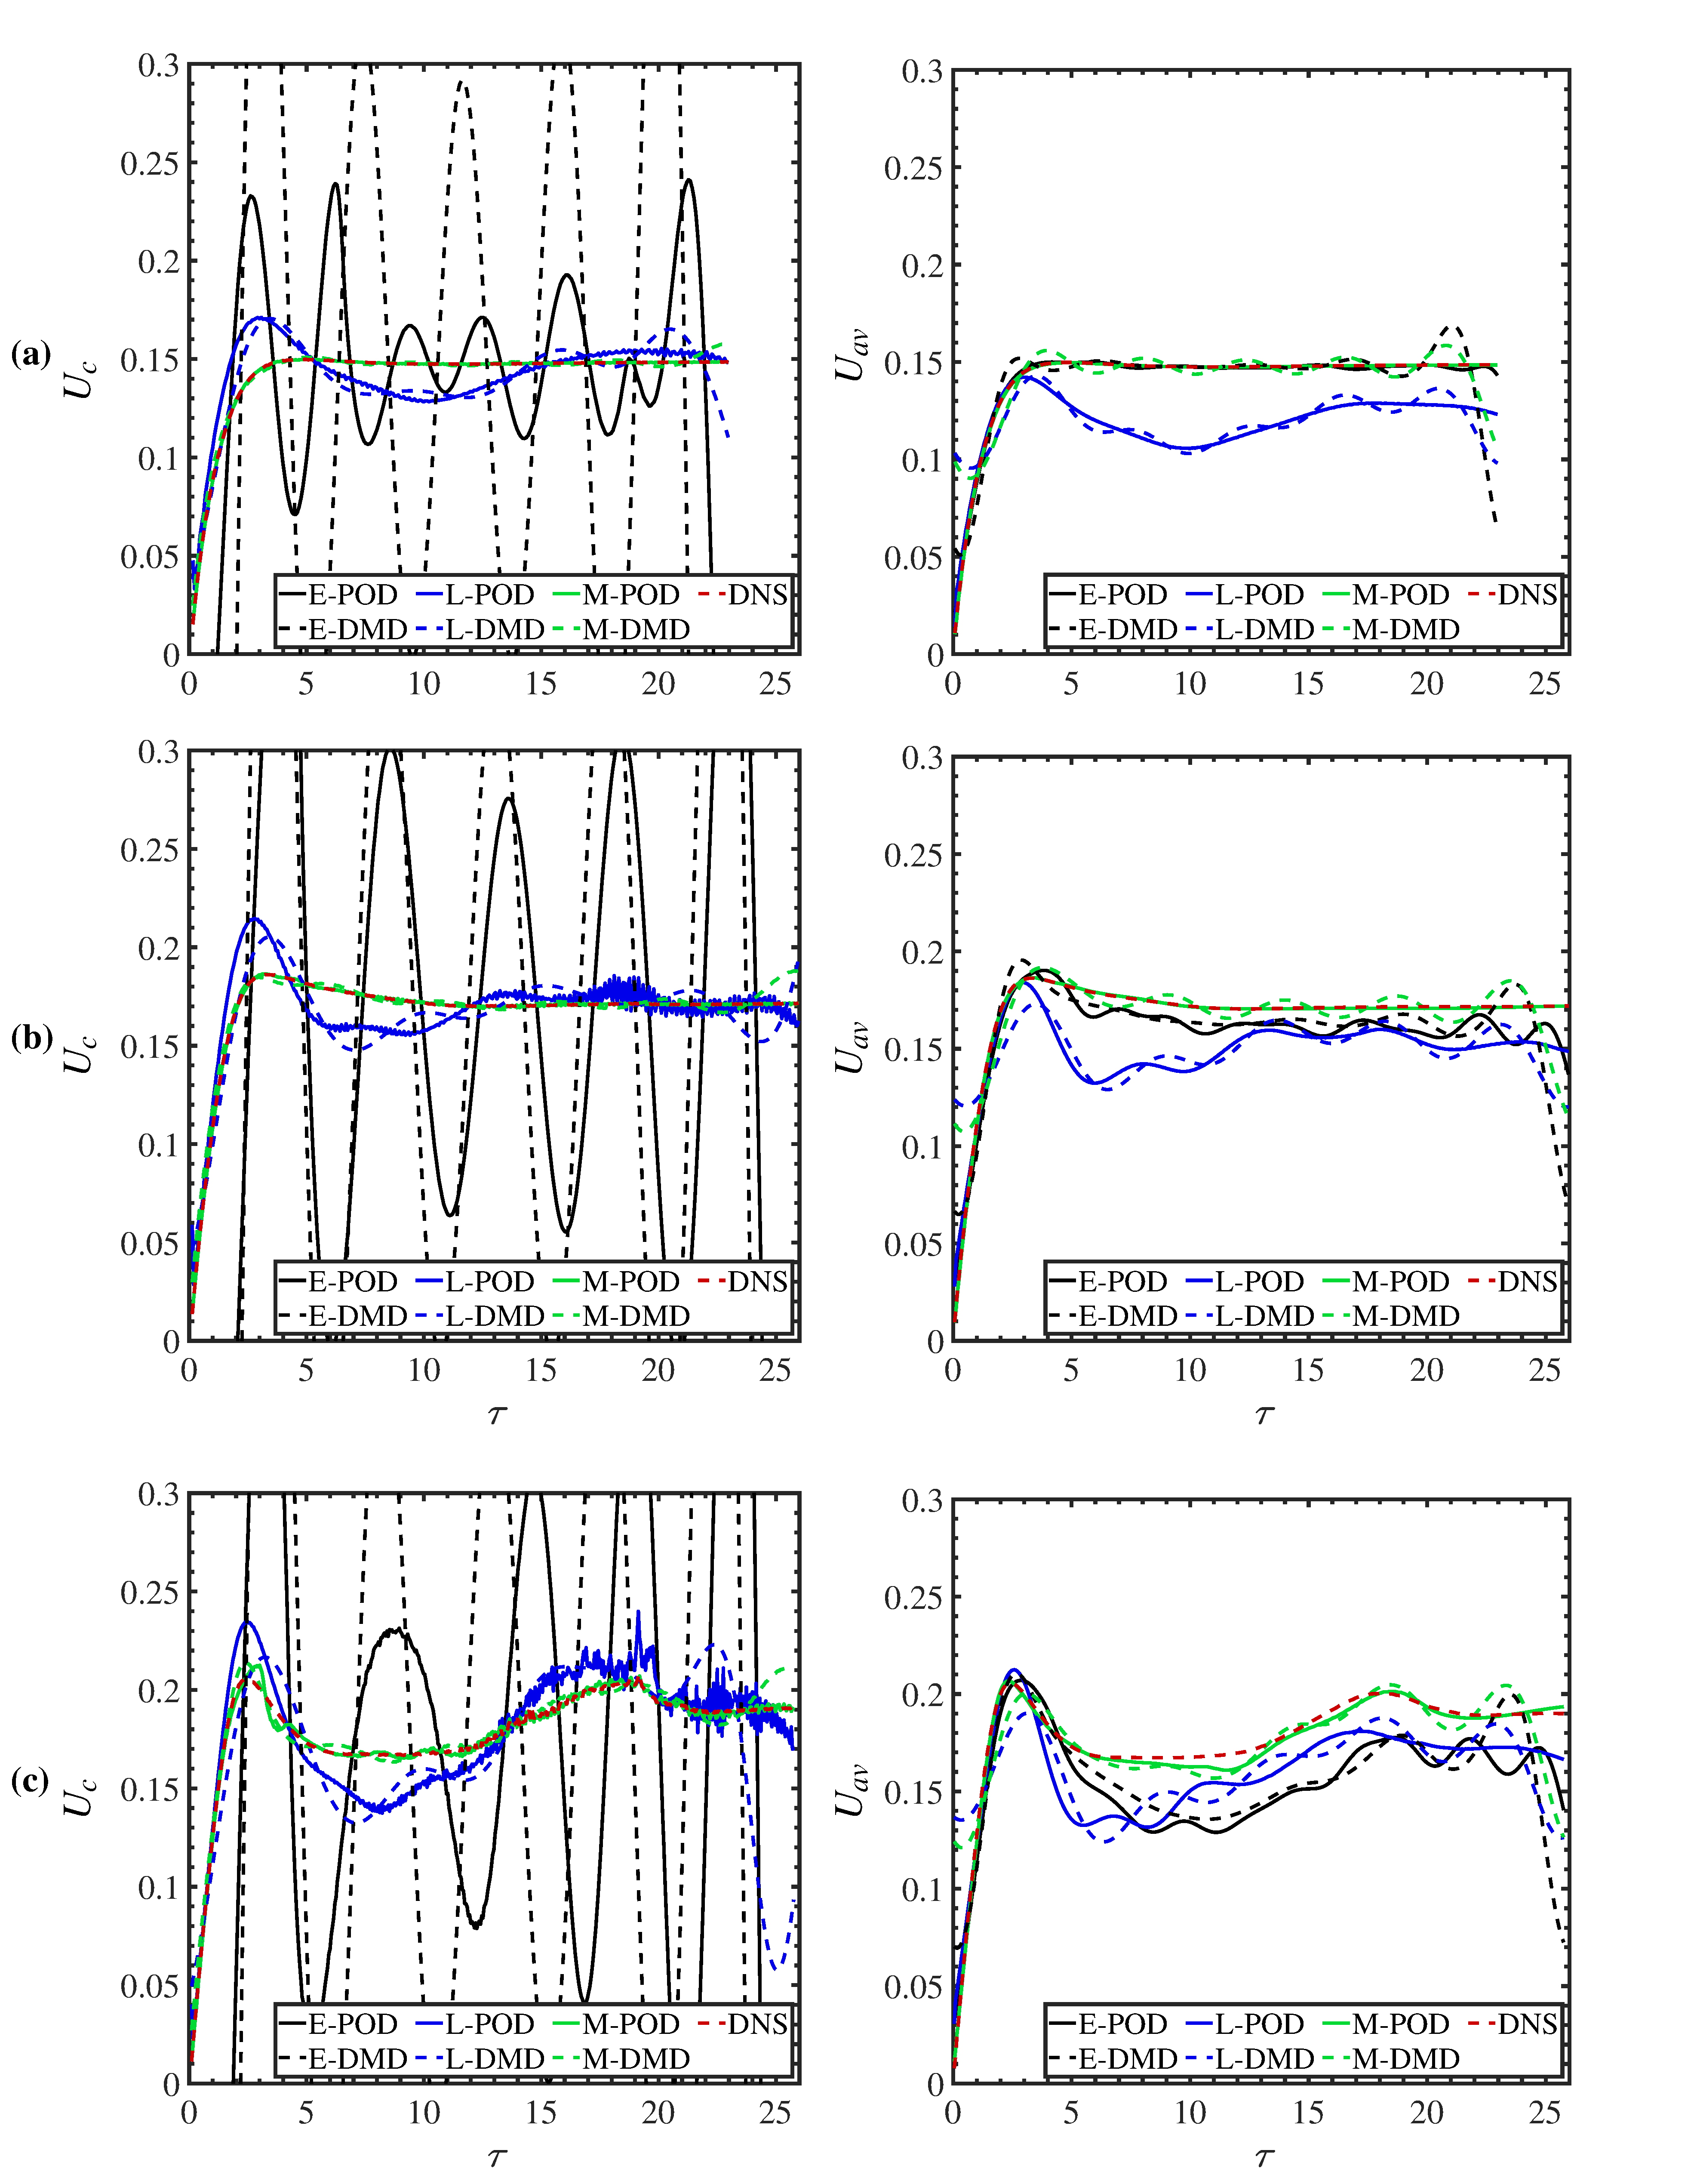
\includegraphics[scale=0.225,trim={0cm 0cm 0cm 0cm},clip]{Figure_6.pdf}
		\caption{Centroid-based rise velocity $U_{\mathrm{c}}$ (left) and average-based rise velocity $U_{\mathrm{av}}$ (right) approximated using 10 modes for cases (a) C$_1$, (b) C$_2$, and (c) C$_3$. The same number of modes is used for the velocity and gas volume fraction fields.}
		\label{Fig6}
	\end{figure}
	
	A widely analysed output parameter associated with rising bubbles is the rise velocity. In the present work, two definitions of rise velocity are evaluated. The first is an average-based quantity obtained directly from the reconstructed velocity field defined as,
	\begin{equation}
		U_{\mathrm{av}}(\tau)=\frac{1}{V_b(\tau)}\int_{V_b(\tau)} U_{\mathrm{rise}}(\mathbf{X},\tau)\,\mathrm{d}V,
	\end{equation}

	\noindent where $U_{\mathrm{rise}}$ denotes the local velocity in the rise direction and $V_b(\tau)$ is the bubble volume. The second is a centroid-based quantity $U_{\mathrm{c}}(\tau)$ obtained as the time derivative of the centroid coordinate in the rise direction, where the centroid-position vector $\mathbf{X}_{\mathrm{cen}}$ is defined in Equation~(\ref{eq Xcen}). In the present implementation, these volume integrals are evaluated using gas volume fraction weighting, yielding the corresponding area-weighted form in 2D axisymmetry and the standard volume average in 3D. Accordingly, two observation fields, including the velocity field and the gas volume fraction field, are required to evaluate the rise velocity. The gas volume fraction reconstruction is used either to define the instantaneous bubble volume and centroid position or to weight the average-based velocity. In contrast, the velocity reconstruction is used directly in the average-based definition. These two quantities are considered because the average-based rise velocity is commonly used in numerical studies, whereas the centroid-based rise velocity is often more accessible in experimental measurements.
	
	The time variation of the rise velocity obtained using different framework-method combinations is compared with DNS for the three cases C$_1$, C$_2$, and C$_3$ in Figure~\ref{Fig6}, where panels (a), (b), and (c) correspond to those cases, respectively. Within each case panel, the left plot shows the centroid-based quantity $U_{\mathrm{c}}$ and the right plot shows the average-based quantity $U_{\mathrm{av}}$. The centroid-based definition is markedly more sensitive to errors in the gas volume fraction because it is the basis for obtaining the centroid location, particularly in the Eulerian frame, where the bubble interface is poorly reconstructed. In the Lagrangian framework, the centroid-based results are improved relative to the Eulerian framework, yet the moving-reference reconstructions remain much more accurate.
	
	Unlike the centroid-based rise velocity, for which the Eulerian framework performs poorly, the average-based rise velocity is reconstructed more accurately in this frame. The Lagrangian reconstruction follows the DNS trend reasonably well during the initial acceleration stage and up to the rise-velocity peak, but it begins to degrade thereafter. The DMD-based reconstructions show large deviations during the early and late stages of the rise process. Overall, the moving-reference framework provides the most reliable estimate of the average-based rise velocity. As the bubble deformation increases in C$_2$ and C$_3$, the efficiency of M-POD becomes more pronounced. The M-POD remains closest to DNS throughout the rise, whereas the Eulerian and DMD-based reconstructions exhibit more pronounced deviations. The average-based rise velocity confirms that M-POD is the most reliable framework-method combination across more complex cases, while M-DMD is the second-best compromise between accuracy and compactness.
	
	Overall, the 2D results show that the moving-reference framework provides the most reliable description of the rise velocity across the three cases, while the Eulerian framework degrades as deformation increases, and the Lagrangian framework performs poorly despite low field reconstruction error. This comparison is summarized quantitatively in Table~\ref{tab:rmsd_summary_all_cases}, which gathers the RMSD values. On this basis, the moving-reference framework is adopted in the following subsection to analyze the 3D cases, as it provides the best balance between low-order compactness and physically meaningful reconstruction of the bubble dynamics.
	
	\subsection{3D cases of a rising bubble}
	
	The last and perhaps most complex scenarios considered in this work are the 3D cases C$_4$ and C$_5$ of a rising, deforming bubble with rectilinear, transition, and oscillatory stages. The moving-reference POD and DMD are considered for reconstructing the rise characteristics. In both C$_4$ and C$_5$, 10 modes are used for all the properties. Figure~\ref{Fig7} summarizes these results, with case C$_4$ shown in the top row and case C$_5$ in the bottom row. Panels (a), (b), (c), and (d) show the 3D rise trajectory, the 2D projection of the rise trajectory, the bubble interface at three intervals, and the sphericity profile, respectively. Additionally, the bubble's rise velocity in 3D space is obtained, and the results are shown in Figure~\ref{Fig8}. A similar discussion to that presented for the 2D bubble in Section~\ref{Bubble interface} is given here for the 3D cases. 
	
	\begin{figure}[pos=!t]
		\centering
			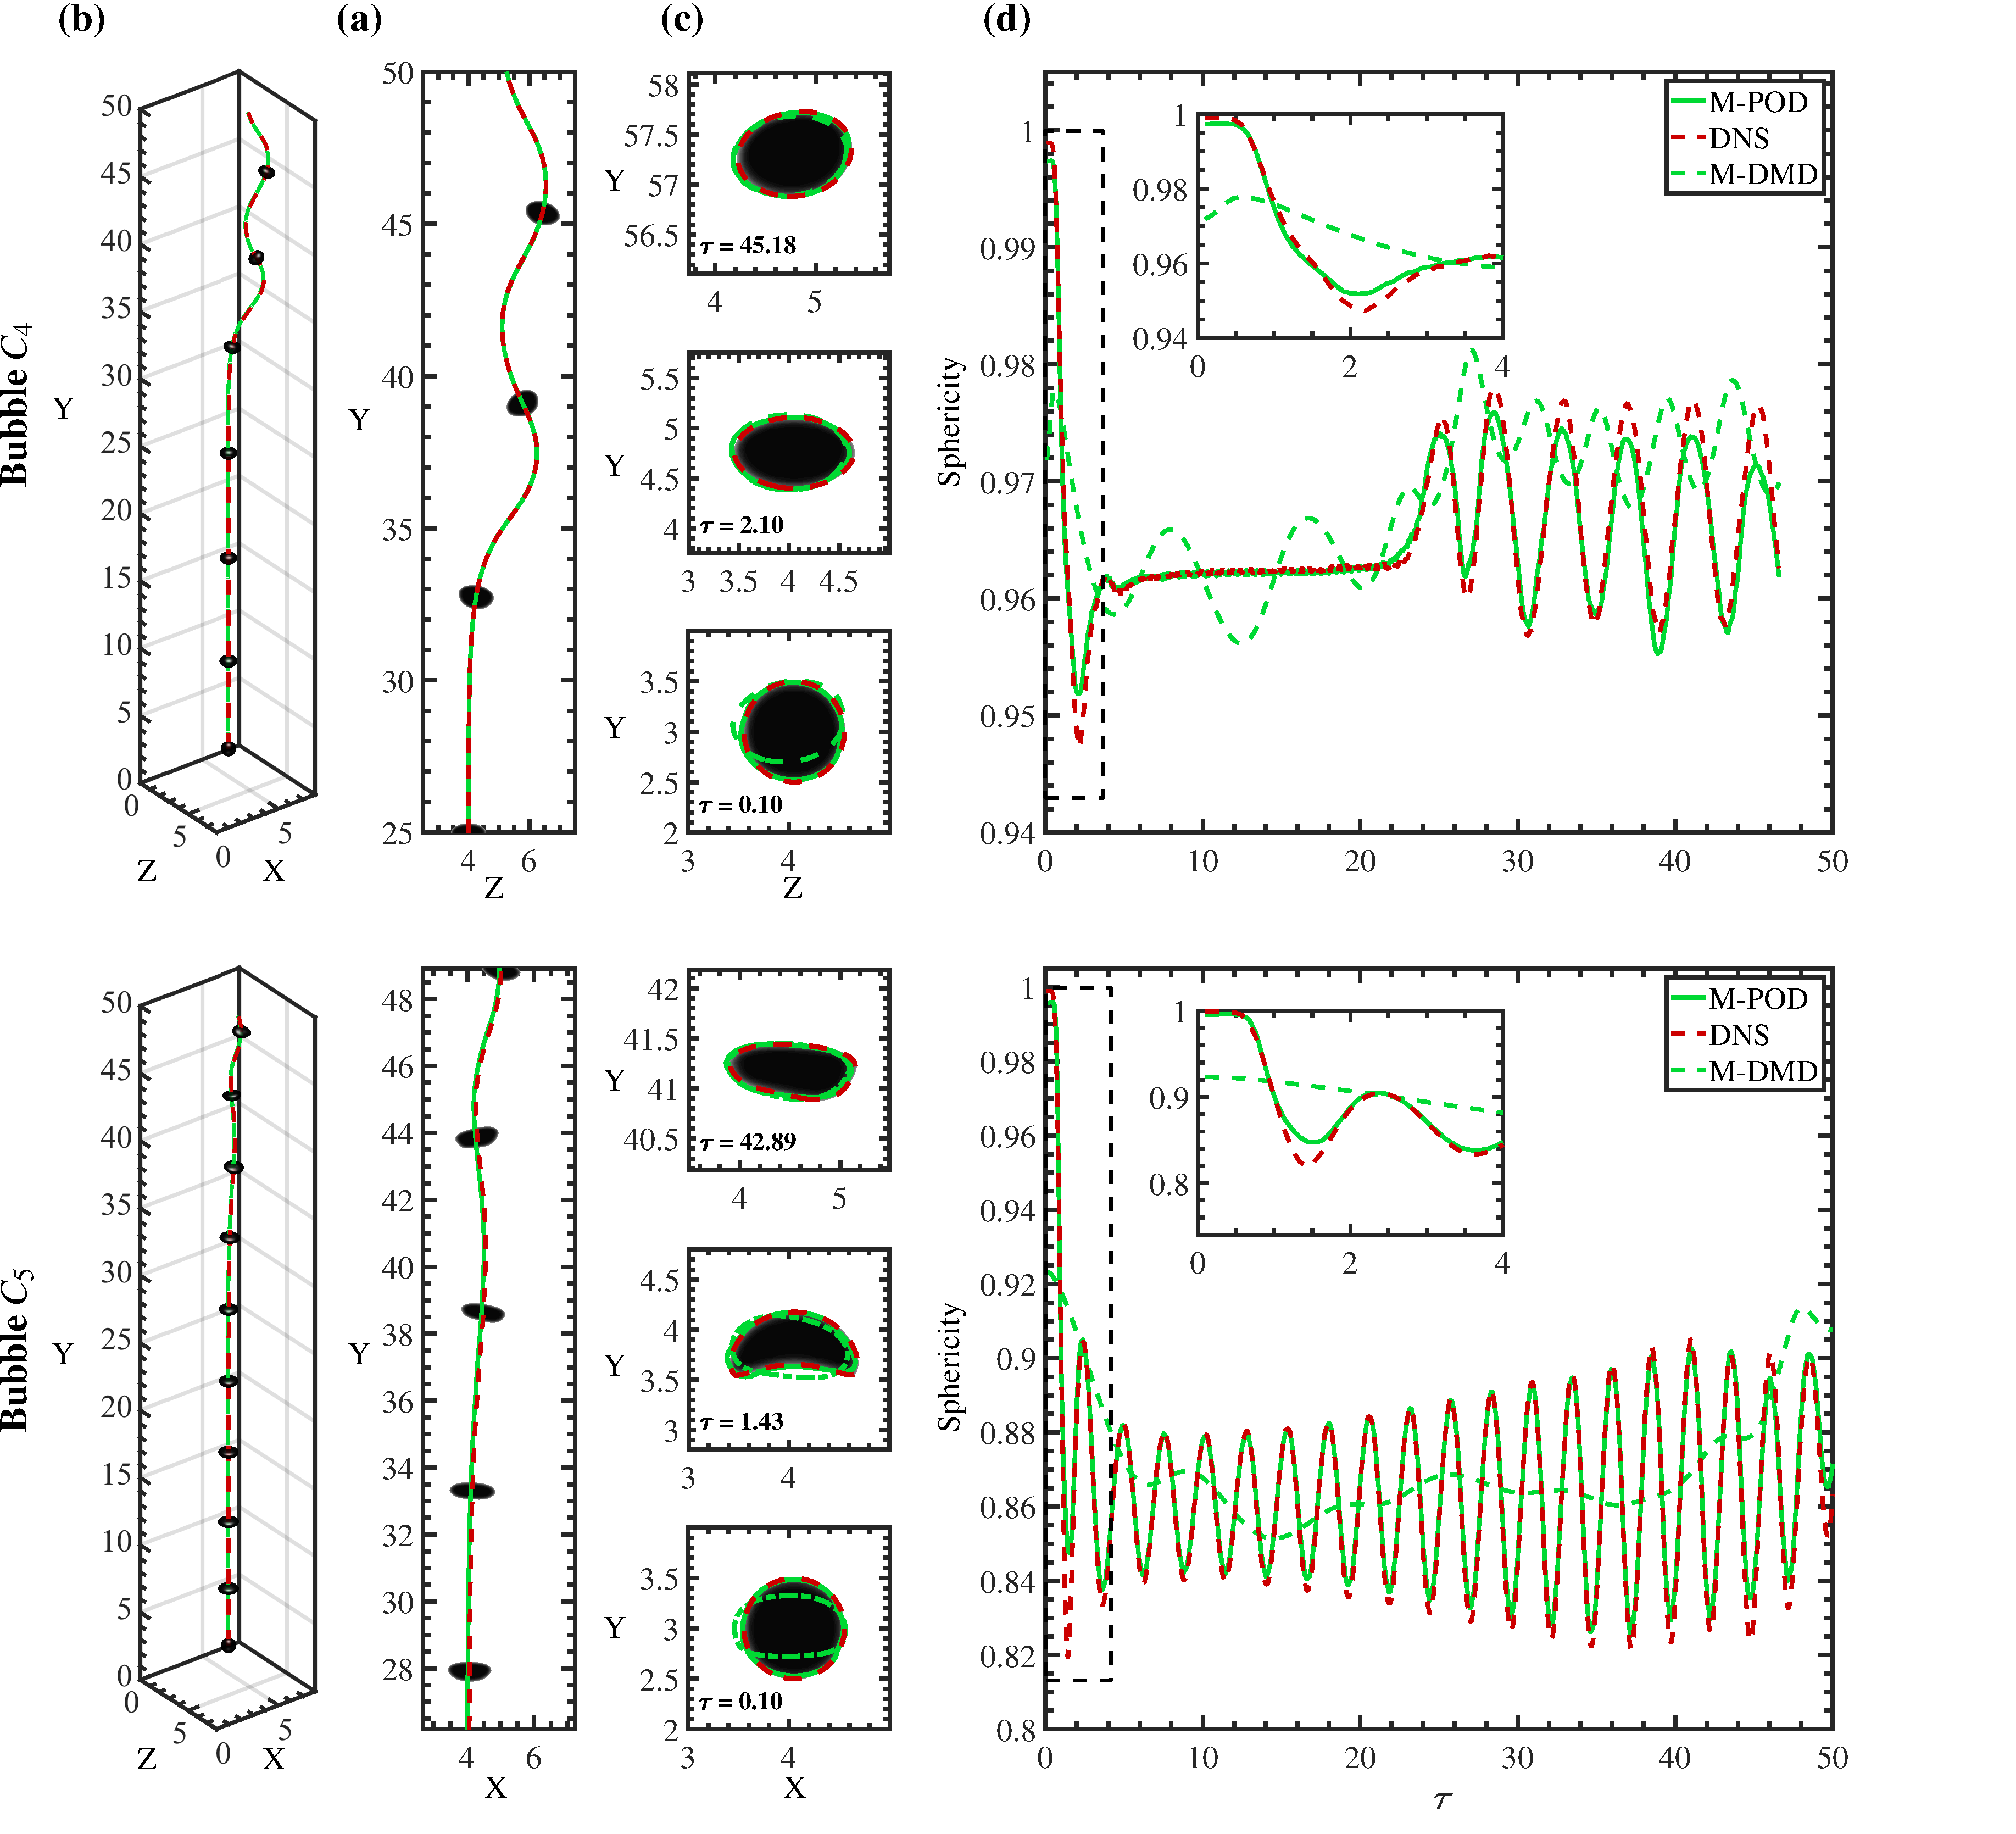
\includegraphics[scale=0.28,trim={0cm 0cm 0cm 0cm},clip]{Figure_7.pdf}
		\caption{Rise characteristics of the 3D bubble cases C$_4$ (top row) and C$_5$ (bottom row) using 10 modes. Panels (a), (b), (c), and (d) show the 3D rise trajectory, the 2D projection of the rise trajectory, the bubble interface at three intervals $\tau_{1}-\tau_{3}$, and the sphericity profile, respectively.}
		\label{Fig7}
	\end{figure}
	
	
	In the case of C$_4$ with less deformation, shown in the top row of Figure~\ref{Fig7}, the 3D rise trajectory shown in panel (a) is reconstructed with high accuracy by both methods. This is consistent with the RMSD values of 0.14\% and 0.15\% for M-POD and M-DMD, respectively. The corresponding 2D projection in panel (b) also remains close to DNS, indicating that the global translational motion is captured well by both methods. The bubble interface shown in panel (c) is depicted as a contour plot at three different instances during the rise process. The bubble interface determined via M-POD remains close to the DNS data, while M-DMD shows more visible deviations. The time variation of the sphericity profile is shown in panel (d), with RMSD errors of 0.16\% and 0.88\% for M-POD and M-DMD, respectively. Similar to the observations in the 2D cases, the deviations of M-DMD are more pronounced in the early stages of the rise, as highlighted by the bubble interface at $\tau_1$ in panel (c), where DMD less accurately captures the spherical shape of the bubble. Overall, the results for C$_4$ indicate that both M-POD and M-DMD can accurately reconstruct the rise trajectory. Still, M-POD provides a more accurate representation of the bubble interface and sphericity.
	
	\begin{figure}[pos=!t]
		\centering
			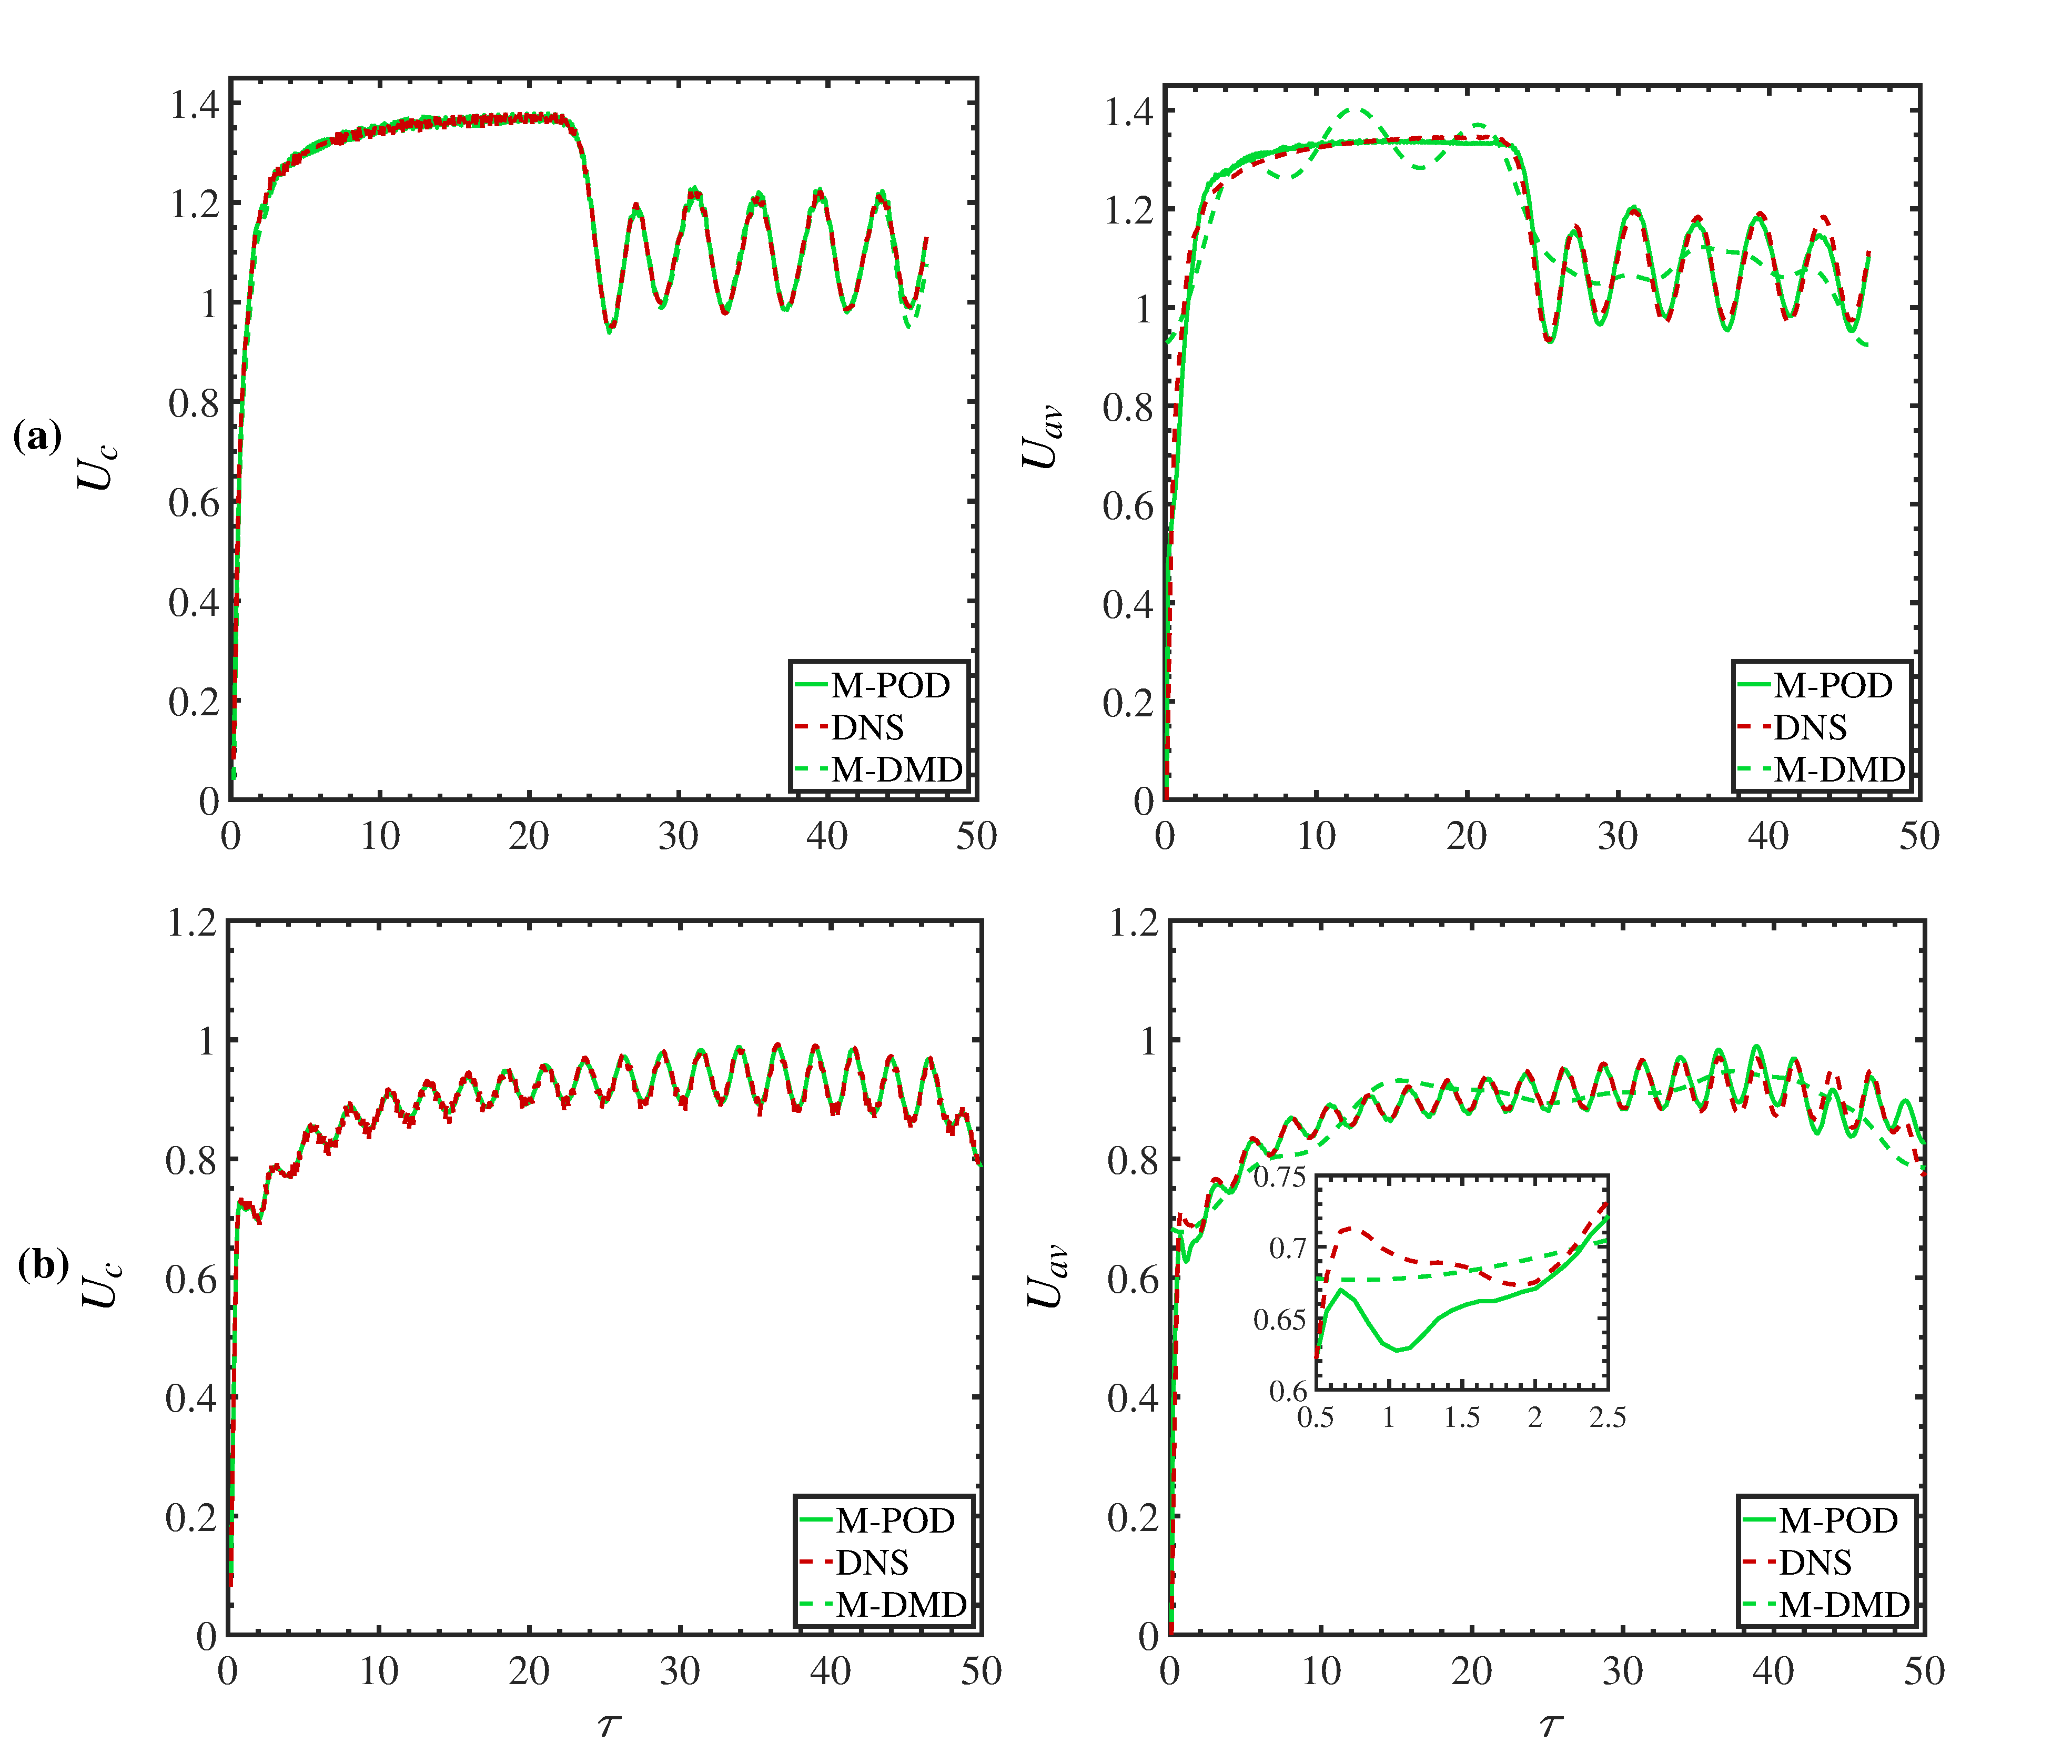
\includegraphics[scale=0.22,trim={0cm 0cm 4cm 0cm},clip]{Figure_8.pdf}
		\caption{Centroid-based rise velocity $U_{\mathrm{c}}$ (left) and average-based rise velocity $U_{\mathrm{av}}$ (right) approximated using 10 modes for cases (a) C$_4$ and (b) C$_5$. The same number of modes is used for the velocity and gas volume fraction fields.}
		\label{Fig8}
	\end{figure}
	
	In the case of C$_5$ with more complex deformation, shown in the bottom row of Figure~\ref{Fig7}, the rise trajectory is still reconstructed accurately by both methods, with RMSD errors of 0.16\% for both M-POD and M-DMD. However, the increased deformation affects the local shape reconstruction more strongly than the global trajectory. The 2D projection and the 3D trajectory remain close to the DNS results, whereas the interface and sphericity show a clearer difference between the methods. The time variation of sphericity shown in panel (d) confirms that M-POD remains close to the DNS, with an RMSD of 0.49\%, slightly larger than C$_4$. M-DMD exhibits noticeably larger deviations, particularly at $\tau_2=1.43$, where the bubble is severely deformed, with an RMSD error of 3.15\%. As in C$_4$, these deviations are most visible in the early stages, highlighted by the insets for each case. Overall, the comparison between C$_4$ and C$_5$ indicates that the reduction in accuracy with increasing deformation is modest for M-POD but much more noticeable for M-DMD, especially for the interface-related quantities.
	
	The rise velocity of the 3D bubbles C$_4$ and C$_5$ is estimated and compared with the DNS values. As illustrated in Figure~\ref{Fig8}, the left plot shows the centroid-based quantity $U_{\mathrm{c}}$ and the right plot shows the average-based quantity $U_{\mathrm{av}}$. In the case of C$_4$, M-POD yields the smaller RMSD for both definitions of rise velocity, namely 0.39\% for the centroid-based quantity and 2.45\% for the average-based quantity, compared with 1.29\% and 7.87\% for M-DMD. For the more complex case C$_5$, both methods give the same centroid-based RMSD of 0.94\%, while M-POD remains more accurate for the average-based rise velocity, with an RMSD error of 2.67\% compared with 6.14\% for M-DMD. The average-based rise velocity is therefore the quantity that more clearly separates the performance of the two methods in 3D, whereas the centroid-based quantity remains comparably accurate for both methods.
	
	In summary, based on the RMSD values reported above, M-POD appears to be the more reliable method for capturing 3D bubble dynamics. In particular, both M-POD and M-DMD reconstruct the rise trajectory with very small error. Still, this global quantity alone is insufficient to distinguish between the quality of the two reconstructions. The clearer separation appears in the more deformation-sensitive local quantities, namely the interface, sphericity, and the average-based rise velocity, for which M-POD remains consistently more accurate. Furthermore, although M-DMD provides high accuracy in approximating the rise trajectory, it is less accurate than M-POD in estimating the rise velocity and interface of the 3D bubble, especially during the early stages of the rise. 
		
	\section{Summary and conclusions}
	\label{Conclusion}
	
	The present work has examined the applicability of classic data-driven methods, specifically POD and DMD with optimized amplitudes, as reduced-order tools for state estimation of five rising bubbles across rectilinear, transitional, and oscillatory regimes within the Eulerian, Lagrangian, and moving-reference frameworks. Two in-house multiphase solvers, SI-LSM$_{\text{col}}$ on an \textit{axisymmetric} coordinate system and CDI on a 3D \textit{Cartesian} coordinate system, were used to obtain the flow-field datasets for five cases used to train the data-driven techniques. The evaluation criteria focused on the relative reconstruction error of the observation fields and the RMSD of key rise characteristics such as interface shape, rise trajectory, and rise velocity. Taken together, these two classes of error show that compact field reconstruction and physically reliable bubble reconstruction are related but not interchangeable criteria. The overall quantitative comparison of RMSD error for the five cases considered in this study is summarized in Table~\ref{tab:rmsd_summary_all_cases}. 
	
	\begin{table}[pos=!t]
		\begin{center}
			\caption{RMSD errors in \% for the reconstructed rise properties of cases C$_1$--C$_5$ using 10 modes. For C$_1$--C$_3$, the reported quantities are the centroid-based rise velocity $U_{\mathrm{c}}$, the average-based rise velocity $U_{\mathrm{av}}$, and circularity. For C$_4$ and C$_5$, the reported quantities are the rise trajectory, the centroid-based rise velocity $U_{\mathrm{c}}$, the average-based rise velocity $U_{\mathrm{av}}$, and sphericity. Dashes indicate combinations that were not reported for the corresponding case.}
			\vspace{0cm}
			\scriptsize
			\setlength{\tabcolsep}{3.2pt}
			\renewcommand{\arraystretch}{1.15}
			\resizebox{\textwidth}{!}{%
				\begin{tabular}{|c|ccc|ccc|ccc|cccc|cccc|}
					\hline\hline
					Method & \multicolumn{3}{c|}{C$_1$} & \multicolumn{3}{c|}{C$_2$} & \multicolumn{3}{c|}{C$_3$} & \multicolumn{4}{c|}{C$_4$} & \multicolumn{4}{c|}{C$_5$} \\
					\hline
					& $U_{\mathrm{c}}$ & $U_{\mathrm{av}}$ & Circ. & $U_{\mathrm{c}}$ & $U_{\mathrm{av}}$ & Circ. & $U_{\mathrm{c}}$ & $U_{\mathrm{av}}$ & Circ. & Traj. & $U_{\mathrm{c}}$ & $U_{\mathrm{av}}$ & Sph. & Traj. & $U_{\mathrm{c}}$ & $U_{\mathrm{av}}$ & Sph. \\
					\hline
					E-POD & 53.81 & 0.95 & 2.75 & 135.00 & 6.33 & 6.82 & 163.08 & 14.75 & 43.49 & -- & -- & -- & -- & -- & -- & -- & -- \\
					\hline
					E-DMD & 310.77 & 9.36 & 4.57 & 320.43 & 10.64 & 7.54 & 321.73 & 16.46 & 50.11 & -- & -- & -- & -- & -- & -- & -- & -- \\
					\hline
					L-POD & 8.96 & 18.46 & 36.65 & 7.21 & 13.62 & 37.41 & 7.85 & 11.67 & 21.82 & -- & -- & -- & -- & -- & -- & -- & -- \\
					\hline
					L-DMD & 8.99 & 20.54 & 39.00 & 7.09 & 16.51 & 38.98 & 19.21 & 15.65 & 28.22 & -- & -- & -- & -- & -- & -- & -- & -- \\
					\hline
					M-POD & 0.07 & 0.16 & 0.13 & 0.20 & 0.32 & 0.27 & 1.23 & 1.72 & 1.42 & 0.14 & 0.39 & 2.45 & 0.16 & 0.16 & 0.94 & 2.67 & 0.49 \\
					\hline
					M-DMD & 1.88 & 8.56 & 0.32 & 2.77 & 8.66 & 2.71 & 3.19 & 9.63 & 6.15 & 0.15 & 1.29 & 7.87 & 0.88 & 0.16 & 0.94 & 6.14 & 3.15 \\
					\hline\hline
				\end{tabular}%
			}
			\label{tab:rmsd_summary_all_cases}
		\end{center}
	\end{table}
	
	The overall assessment of the relative reconstruction error shows that the choice of reference frame has a stronger influence on reconstruction efficiency than the choice between POD and DMD. In terms of field compactness, the Lagrangian and moving-reference frameworks consistently outperform the Eulerian one, while within a given framework, POD remains the more accurate low-order method. The analysis also showed that the velocity field is more low-dimensional than the gas volume fraction field in the Eulerian and moving-reference frameworks. In addition, largely deformed bubbles showed a slightly higher relative field reconstruction error than simple bubbles, yet their errors remained below 2\%. 
	
	Subsequent analysis of circularity and rise velocity for the \textit{axisymmetric} cases demonstrates that field compactness alone is not sufficient to assess physical reliability. In particular, the Lagrangian framework is the most compact for field reconstruction, though it is not the most reliable for reconstructed rise characteristics. In the moving-reference framework, however, the most accurate interface and rise velocity is achieved. 
	
	The results for the rising bubble with an oscillatory trajectory on the 3D \textit{Cartesian} coordinate system reveal that M-POD and M-DMD can reconstruct the rise trajectory with acceptable accuracy. However, similar to the limitation observed in the \textit{axisymmetric} cases, DMD is less accurate for the more deformation-sensitive quantities. Sphericity and the average-based rise velocity provide a much more discriminating assessment of reconstruction quality. At the same fixed rank of 10 modes used in the 3D comparison, M-POD remains more accurate than M-DMD for these local rise characteristics. Collectively, the moving-reference POD is the recommended reduced-order tool for studying a rising bubble.
	
	The present work has shown that, within a moving-reference framework, a rising bubble and its key rise characteristics can be represented accurately at a fixed low-order level using as few as 10 modes. The findings are a strong motivation to study more complex Lagrangian-evolving flow features, particularly wake structures behind the bubble, such as toroidal vortices, by first representing them in a moving reference frame, then decomposing them into modes, and subsequently analysing their dynamics. In the future, M-POD may also be extended to more complex processes, such as bubble breakup or coalescence, through a more detailed investigation of the dominant modes. More generally, the same frame-change idea may be applied to other problems where translational motion and transient phenomena dominate the flow, and it may also be combined with other data-driven techniques, such as high-order DMD, to evaluate their performance. \\
	
	{\noindent \bf{Funding}} \\
	
	The work was supported by the Research Council of Norway (NRC) (Grant no. 334652). The computations were performed on resources provided by Sigma2\textemdash the National Infrastructure for High-Performance Computing and Data Storage in Norway with project number NN9646K.\\
	\\
	{\bf{Conflict of interest}} \\
	
	The authors declare no conflict of interest. \\
	\\
	{\bf{Data availability}} \\
	

	The data that support the findings of this study are available from the corresponding author upon reasonable request. \\
	
\nolinenumbers

\bibliographystyle{elsarticle-num-names}
\bibliography{library}
	
	
\end{document}

